% Options for packages loaded elsewhere
\PassOptionsToPackage{unicode}{hyperref}
\PassOptionsToPackage{hyphens}{url}
%
\documentclass[
]{article}
\usepackage{amsmath,amssymb}
\usepackage{iftex}
\ifPDFTeX
  \usepackage[T1]{fontenc}
  \usepackage[utf8]{inputenc}
  \usepackage{textcomp} % provide euro and other symbols
\else % if luatex or xetex
  \usepackage{unicode-math} % this also loads fontspec
  \defaultfontfeatures{Scale=MatchLowercase}
  \defaultfontfeatures[\rmfamily]{Ligatures=TeX,Scale=1}
\fi
\usepackage{lmodern}
\ifPDFTeX\else
  % xetex/luatex font selection
\fi
% Use upquote if available, for straight quotes in verbatim environments
\IfFileExists{upquote.sty}{\usepackage{upquote}}{}
\IfFileExists{microtype.sty}{% use microtype if available
  \usepackage[]{microtype}
  \UseMicrotypeSet[protrusion]{basicmath} % disable protrusion for tt fonts
}{}
\makeatletter
\@ifundefined{KOMAClassName}{% if non-KOMA class
  \IfFileExists{parskip.sty}{%
    \usepackage{parskip}
  }{% else
    \setlength{\parindent}{0pt}
    \setlength{\parskip}{6pt plus 2pt minus 1pt}}
}{% if KOMA class
  \KOMAoptions{parskip=half}}
\makeatother
\usepackage{xcolor}
\usepackage[margin=1in]{geometry}
\usepackage{color}
\usepackage{fancyvrb}
\newcommand{\VerbBar}{|}
\newcommand{\VERB}{\Verb[commandchars=\\\{\}]}
\DefineVerbatimEnvironment{Highlighting}{Verbatim}{commandchars=\\\{\}}
% Add ',fontsize=\small' for more characters per line
\usepackage{framed}
\definecolor{shadecolor}{RGB}{248,248,248}
\newenvironment{Shaded}{\begin{snugshade}}{\end{snugshade}}
\newcommand{\AlertTok}[1]{\textcolor[rgb]{0.94,0.16,0.16}{#1}}
\newcommand{\AnnotationTok}[1]{\textcolor[rgb]{0.56,0.35,0.01}{\textbf{\textit{#1}}}}
\newcommand{\AttributeTok}[1]{\textcolor[rgb]{0.13,0.29,0.53}{#1}}
\newcommand{\BaseNTok}[1]{\textcolor[rgb]{0.00,0.00,0.81}{#1}}
\newcommand{\BuiltInTok}[1]{#1}
\newcommand{\CharTok}[1]{\textcolor[rgb]{0.31,0.60,0.02}{#1}}
\newcommand{\CommentTok}[1]{\textcolor[rgb]{0.56,0.35,0.01}{\textit{#1}}}
\newcommand{\CommentVarTok}[1]{\textcolor[rgb]{0.56,0.35,0.01}{\textbf{\textit{#1}}}}
\newcommand{\ConstantTok}[1]{\textcolor[rgb]{0.56,0.35,0.01}{#1}}
\newcommand{\ControlFlowTok}[1]{\textcolor[rgb]{0.13,0.29,0.53}{\textbf{#1}}}
\newcommand{\DataTypeTok}[1]{\textcolor[rgb]{0.13,0.29,0.53}{#1}}
\newcommand{\DecValTok}[1]{\textcolor[rgb]{0.00,0.00,0.81}{#1}}
\newcommand{\DocumentationTok}[1]{\textcolor[rgb]{0.56,0.35,0.01}{\textbf{\textit{#1}}}}
\newcommand{\ErrorTok}[1]{\textcolor[rgb]{0.64,0.00,0.00}{\textbf{#1}}}
\newcommand{\ExtensionTok}[1]{#1}
\newcommand{\FloatTok}[1]{\textcolor[rgb]{0.00,0.00,0.81}{#1}}
\newcommand{\FunctionTok}[1]{\textcolor[rgb]{0.13,0.29,0.53}{\textbf{#1}}}
\newcommand{\ImportTok}[1]{#1}
\newcommand{\InformationTok}[1]{\textcolor[rgb]{0.56,0.35,0.01}{\textbf{\textit{#1}}}}
\newcommand{\KeywordTok}[1]{\textcolor[rgb]{0.13,0.29,0.53}{\textbf{#1}}}
\newcommand{\NormalTok}[1]{#1}
\newcommand{\OperatorTok}[1]{\textcolor[rgb]{0.81,0.36,0.00}{\textbf{#1}}}
\newcommand{\OtherTok}[1]{\textcolor[rgb]{0.56,0.35,0.01}{#1}}
\newcommand{\PreprocessorTok}[1]{\textcolor[rgb]{0.56,0.35,0.01}{\textit{#1}}}
\newcommand{\RegionMarkerTok}[1]{#1}
\newcommand{\SpecialCharTok}[1]{\textcolor[rgb]{0.81,0.36,0.00}{\textbf{#1}}}
\newcommand{\SpecialStringTok}[1]{\textcolor[rgb]{0.31,0.60,0.02}{#1}}
\newcommand{\StringTok}[1]{\textcolor[rgb]{0.31,0.60,0.02}{#1}}
\newcommand{\VariableTok}[1]{\textcolor[rgb]{0.00,0.00,0.00}{#1}}
\newcommand{\VerbatimStringTok}[1]{\textcolor[rgb]{0.31,0.60,0.02}{#1}}
\newcommand{\WarningTok}[1]{\textcolor[rgb]{0.56,0.35,0.01}{\textbf{\textit{#1}}}}
\usepackage{graphicx}
\makeatletter
\def\maxwidth{\ifdim\Gin@nat@width>\linewidth\linewidth\else\Gin@nat@width\fi}
\def\maxheight{\ifdim\Gin@nat@height>\textheight\textheight\else\Gin@nat@height\fi}
\makeatother
% Scale images if necessary, so that they will not overflow the page
% margins by default, and it is still possible to overwrite the defaults
% using explicit options in \includegraphics[width, height, ...]{}
\setkeys{Gin}{width=\maxwidth,height=\maxheight,keepaspectratio}
% Set default figure placement to htbp
\makeatletter
\def\fps@figure{htbp}
\makeatother
\setlength{\emergencystretch}{3em} % prevent overfull lines
\providecommand{\tightlist}{%
  \setlength{\itemsep}{0pt}\setlength{\parskip}{0pt}}
\setcounter{secnumdepth}{-\maxdimen} % remove section numbering
\ifLuaTeX
  \usepackage{selnolig}  % disable illegal ligatures
\fi
\IfFileExists{bookmark.sty}{\usepackage{bookmark}}{\usepackage{hyperref}}
\IfFileExists{xurl.sty}{\usepackage{xurl}}{} % add URL line breaks if available
\urlstyle{same}
\hypersetup{
  pdftitle={Final\_Project},
  pdfauthor={S/17/436},
  hidelinks,
  pdfcreator={LaTeX via pandoc}}

\title{Final\_Project}
\author{S/17/436}
\date{2023-11-14}

\begin{document}
\maketitle

\hypertarget{required-packages}{%
\section{Required Packages}\label{required-packages}}

\begin{Shaded}
\begin{Highlighting}[]
\FunctionTok{library}\NormalTok{(tidyverse)}
\end{Highlighting}
\end{Shaded}

\begin{verbatim}
## Warning: package 'tidyverse' was built under R version 4.3.2
\end{verbatim}

\begin{verbatim}
## Warning: package 'ggplot2' was built under R version 4.3.2
\end{verbatim}

\begin{verbatim}
## -- Attaching core tidyverse packages ------------------------ tidyverse 2.0.0 --
## v dplyr     1.1.3     v readr     2.1.4
## v forcats   1.0.0     v stringr   1.5.0
## v ggplot2   3.4.4     v tibble    3.2.1
## v lubridate 1.9.2     v tidyr     1.3.0
## v purrr     1.0.2     
## -- Conflicts ------------------------------------------ tidyverse_conflicts() --
## x dplyr::filter() masks stats::filter()
## x dplyr::lag()    masks stats::lag()
## i Use the conflicted package (<http://conflicted.r-lib.org/>) to force all conflicts to become errors
\end{verbatim}

\begin{Shaded}
\begin{Highlighting}[]
\FunctionTok{library}\NormalTok{(tinytex)}
\end{Highlighting}
\end{Shaded}

\begin{verbatim}
## Warning: package 'tinytex' was built under R version 4.3.2
\end{verbatim}

\begin{Shaded}
\begin{Highlighting}[]
\FunctionTok{library}\NormalTok{(ggplot2)}
\FunctionTok{library}\NormalTok{(corrplot)}
\end{Highlighting}
\end{Shaded}

\begin{verbatim}
## Warning: package 'corrplot' was built under R version 4.3.2
\end{verbatim}

\begin{verbatim}
## corrplot 0.92 loaded
\end{verbatim}

\hypertarget{import-dataset}{%
\section{Import Dataset}\label{import-dataset}}

\begin{Shaded}
\begin{Highlighting}[]
\NormalTok{stroke }\OtherTok{\textless{}{-}} \FunctionTok{read\_csv}\NormalTok{(}\StringTok{\textquotesingle{}../Data/healthcare{-}dataset{-}stroke{-}data.csv\textquotesingle{}}\NormalTok{)}
\end{Highlighting}
\end{Shaded}

\begin{verbatim}
## Rows: 5110 Columns: 12
## -- Column specification --------------------------------------------------------
## Delimiter: ","
## chr (6): gender, ever_married, work_type, Residence_type, bmi, smoking_status
## dbl (6): id, age, hypertension, heart_disease, avg_glucose_level, stroke
## 
## i Use `spec()` to retrieve the full column specification for this data.
## i Specify the column types or set `show_col_types = FALSE` to quiet this message.
\end{verbatim}

\begin{Shaded}
\begin{Highlighting}[]
\CommentTok{\#View(stroke)}
\end{Highlighting}
\end{Shaded}

\begin{Shaded}
\begin{Highlighting}[]
\DocumentationTok{\#\# Display head of the dataset}
\FunctionTok{head}\NormalTok{(stroke)}
\end{Highlighting}
\end{Shaded}

\begin{verbatim}
## # A tibble: 6 x 12
##      id gender   age hypertension heart_disease ever_married work_type    
##   <dbl> <chr>  <dbl>        <dbl>         <dbl> <chr>        <chr>        
## 1  9046 Male      67            0             1 Yes          Private      
## 2 51676 Female    61            0             0 Yes          Self-employed
## 3 31112 Male      80            0             1 Yes          Private      
## 4 60182 Female    49            0             0 Yes          Private      
## 5  1665 Female    79            1             0 Yes          Self-employed
## 6 56669 Male      81            0             0 Yes          Private      
## # i 5 more variables: Residence_type <chr>, avg_glucose_level <dbl>, bmi <chr>,
## #   smoking_status <chr>, stroke <dbl>
\end{verbatim}

\begin{Shaded}
\begin{Highlighting}[]
\DocumentationTok{\#\# Look at the structure of the variables }
\FunctionTok{str}\NormalTok{(stroke)}
\end{Highlighting}
\end{Shaded}

\begin{verbatim}
## spc_tbl_ [5,110 x 12] (S3: spec_tbl_df/tbl_df/tbl/data.frame)
##  $ id               : num [1:5110] 9046 51676 31112 60182 1665 ...
##  $ gender           : chr [1:5110] "Male" "Female" "Male" "Female" ...
##  $ age              : num [1:5110] 67 61 80 49 79 81 74 69 59 78 ...
##  $ hypertension     : num [1:5110] 0 0 0 0 1 0 1 0 0 0 ...
##  $ heart_disease    : num [1:5110] 1 0 1 0 0 0 1 0 0 0 ...
##  $ ever_married     : chr [1:5110] "Yes" "Yes" "Yes" "Yes" ...
##  $ work_type        : chr [1:5110] "Private" "Self-employed" "Private" "Private" ...
##  $ Residence_type   : chr [1:5110] "Urban" "Rural" "Rural" "Urban" ...
##  $ avg_glucose_level: num [1:5110] 229 202 106 171 174 ...
##  $ bmi              : chr [1:5110] "36.6" "N/A" "32.5" "34.4" ...
##  $ smoking_status   : chr [1:5110] "formerly smoked" "never smoked" "never smoked" "smokes" ...
##  $ stroke           : num [1:5110] 1 1 1 1 1 1 1 1 1 1 ...
##  - attr(*, "spec")=
##   .. cols(
##   ..   id = col_double(),
##   ..   gender = col_character(),
##   ..   age = col_double(),
##   ..   hypertension = col_double(),
##   ..   heart_disease = col_double(),
##   ..   ever_married = col_character(),
##   ..   work_type = col_character(),
##   ..   Residence_type = col_character(),
##   ..   avg_glucose_level = col_double(),
##   ..   bmi = col_character(),
##   ..   smoking_status = col_character(),
##   ..   stroke = col_double()
##   .. )
##  - attr(*, "problems")=<externalptr>
\end{verbatim}

\begin{Shaded}
\begin{Highlighting}[]
\DocumentationTok{\#\# Describe the dataset}
\FunctionTok{glimpse}\NormalTok{(stroke)}
\end{Highlighting}
\end{Shaded}

\begin{verbatim}
## Rows: 5,110
## Columns: 12
## $ id                <dbl> 9046, 51676, 31112, 60182, 1665, 56669, 53882, 10434~
## $ gender            <chr> "Male", "Female", "Male", "Female", "Female", "Male"~
## $ age               <dbl> 67, 61, 80, 49, 79, 81, 74, 69, 59, 78, 81, 61, 54, ~
## $ hypertension      <dbl> 0, 0, 0, 0, 1, 0, 1, 0, 0, 0, 1, 0, 0, 0, 0, 1, 0, 1~
## $ heart_disease     <dbl> 1, 0, 1, 0, 0, 0, 1, 0, 0, 0, 0, 1, 0, 1, 1, 0, 1, 0~
## $ ever_married      <chr> "Yes", "Yes", "Yes", "Yes", "Yes", "Yes", "Yes", "No~
## $ work_type         <chr> "Private", "Self-employed", "Private", "Private", "S~
## $ Residence_type    <chr> "Urban", "Rural", "Rural", "Urban", "Rural", "Urban"~
## $ avg_glucose_level <dbl> 228.69, 202.21, 105.92, 171.23, 174.12, 186.21, 70.0~
## $ bmi               <chr> "36.6", "N/A", "32.5", "34.4", "24", "29", "27.4", "~
## $ smoking_status    <chr> "formerly smoked", "never smoked", "never smoked", "~
## $ stroke            <dbl> 1, 1, 1, 1, 1, 1, 1, 1, 1, 1, 1, 1, 1, 1, 1, 1, 1, 1~
\end{verbatim}

\begin{Shaded}
\begin{Highlighting}[]
\DocumentationTok{\#\# Find the dimension of the dataset}
\FunctionTok{dim}\NormalTok{(stroke)}
\end{Highlighting}
\end{Shaded}

\begin{verbatim}
## [1] 5110   12
\end{verbatim}

\hypertarget{data-cleaning}{%
\section{Data Cleaning}\label{data-cleaning}}

\begin{Shaded}
\begin{Highlighting}[]
\CommentTok{\# Count missing values in each column}
\NormalTok{null\_counts }\OtherTok{\textless{}{-}} \FunctionTok{colSums}\NormalTok{(}\FunctionTok{is.na}\NormalTok{(stroke))}

\CommentTok{\# Convert the result to a data frame with column name "Null count"}
\NormalTok{result }\OtherTok{\textless{}{-}} \FunctionTok{data.frame}\NormalTok{(}\StringTok{"Null count"} \OtherTok{=}\NormalTok{ null\_counts)}

\CommentTok{\# Print the result}
\FunctionTok{print}\NormalTok{(result)}
\end{Highlighting}
\end{Shaded}

\begin{verbatim}
##                   Null.count
## id                         0
## gender                     0
## age                        0
## hypertension               0
## heart_disease              0
## ever_married               0
## work_type                  0
## Residence_type             0
## avg_glucose_level          0
## bmi                        0
## smoking_status             0
## stroke                     0
\end{verbatim}

\begin{Shaded}
\begin{Highlighting}[]
\CommentTok{\# Identify "N/A" values}
\NormalTok{na\_indices }\OtherTok{\textless{}{-}} \FunctionTok{lapply}\NormalTok{(stroke, }\ControlFlowTok{function}\NormalTok{(x) }\FunctionTok{which}\NormalTok{(x }\SpecialCharTok{==} \StringTok{"N/A"}\NormalTok{))}

\CommentTok{\# Replace "N/A" values with NA and count missing values}
\NormalTok{missing\_counts }\OtherTok{\textless{}{-}} \FunctionTok{sapply}\NormalTok{(}\DecValTok{1}\SpecialCharTok{:}\FunctionTok{ncol}\NormalTok{(stroke), }\ControlFlowTok{function}\NormalTok{(i) \{}
\NormalTok{  stroke[[i]][na\_indices[[i]]] }\OtherTok{\textless{}{-}} \ConstantTok{NA}
  \FunctionTok{sum}\NormalTok{(}\FunctionTok{is.na}\NormalTok{(stroke[[i]]))}
\NormalTok{\})}

\CommentTok{\# Create a data frame with column names and missing counts}
\NormalTok{result }\OtherTok{\textless{}{-}} \FunctionTok{data.frame}\NormalTok{(}
  \AttributeTok{Column =} \FunctionTok{names}\NormalTok{(stroke),}
  \AttributeTok{Missing\_Count =}\NormalTok{ missing\_counts}
\NormalTok{)}

\CommentTok{\# Print the result}
\FunctionTok{print}\NormalTok{(result)}
\end{Highlighting}
\end{Shaded}

\begin{verbatim}
##               Column Missing_Count
## 1                 id             0
## 2             gender             0
## 3                age             0
## 4       hypertension             0
## 5      heart_disease             0
## 6       ever_married             0
## 7          work_type             0
## 8     Residence_type             0
## 9  avg_glucose_level             0
## 10               bmi           201
## 11    smoking_status             0
## 12            stroke             0
\end{verbatim}

\begin{Shaded}
\begin{Highlighting}[]
\CommentTok{\# Convert column A to numeric and fill missing values with the mean}
\NormalTok{stroke}\SpecialCharTok{$}\NormalTok{bmi }\OtherTok{\textless{}{-}} \FunctionTok{as.numeric}\NormalTok{(}\FunctionTok{as.character}\NormalTok{(stroke}\SpecialCharTok{$}\NormalTok{bmi))}
\end{Highlighting}
\end{Shaded}

\begin{verbatim}
## Warning: NAs introduced by coercion
\end{verbatim}

\begin{Shaded}
\begin{Highlighting}[]
\NormalTok{mean\_A }\OtherTok{\textless{}{-}} \FunctionTok{mean}\NormalTok{(stroke}\SpecialCharTok{$}\NormalTok{bmi, }\AttributeTok{na.rm =} \ConstantTok{TRUE}\NormalTok{)}

\CommentTok{\# Replace missing values in column A with the mean}
\NormalTok{stroke}\SpecialCharTok{$}\NormalTok{bmi[}\FunctionTok{is.na}\NormalTok{(stroke}\SpecialCharTok{$}\NormalTok{bmi)] }\OtherTok{\textless{}{-}}\NormalTok{ mean\_A}

\CommentTok{\# Print the corrected data}
\FunctionTok{print}\NormalTok{(stroke)}
\end{Highlighting}
\end{Shaded}

\begin{verbatim}
## # A tibble: 5,110 x 12
##       id gender   age hypertension heart_disease ever_married work_type    
##    <dbl> <chr>  <dbl>        <dbl>         <dbl> <chr>        <chr>        
##  1  9046 Male      67            0             1 Yes          Private      
##  2 51676 Female    61            0             0 Yes          Self-employed
##  3 31112 Male      80            0             1 Yes          Private      
##  4 60182 Female    49            0             0 Yes          Private      
##  5  1665 Female    79            1             0 Yes          Self-employed
##  6 56669 Male      81            0             0 Yes          Private      
##  7 53882 Male      74            1             1 Yes          Private      
##  8 10434 Female    69            0             0 No           Private      
##  9 27419 Female    59            0             0 Yes          Private      
## 10 60491 Female    78            0             0 Yes          Private      
## # i 5,100 more rows
## # i 5 more variables: Residence_type <chr>, avg_glucose_level <dbl>, bmi <dbl>,
## #   smoking_status <chr>, stroke <dbl>
\end{verbatim}

\hypertarget{exploratory-data-analysis}{%
\section{Exploratory Data Analysis}\label{exploratory-data-analysis}}

\begin{Shaded}
\begin{Highlighting}[]
\CommentTok{\# Display summary statistics}
\FunctionTok{summary}\NormalTok{(stroke)}
\end{Highlighting}
\end{Shaded}

\begin{verbatim}
##        id           gender               age         hypertension    
##  Min.   :   67   Length:5110        Min.   : 0.08   Min.   :0.00000  
##  1st Qu.:17741   Class :character   1st Qu.:25.00   1st Qu.:0.00000  
##  Median :36932   Mode  :character   Median :45.00   Median :0.00000  
##  Mean   :36518                      Mean   :43.23   Mean   :0.09746  
##  3rd Qu.:54682                      3rd Qu.:61.00   3rd Qu.:0.00000  
##  Max.   :72940                      Max.   :82.00   Max.   :1.00000  
##  heart_disease     ever_married        work_type         Residence_type    
##  Min.   :0.00000   Length:5110        Length:5110        Length:5110       
##  1st Qu.:0.00000   Class :character   Class :character   Class :character  
##  Median :0.00000   Mode  :character   Mode  :character   Mode  :character  
##  Mean   :0.05401                                                           
##  3rd Qu.:0.00000                                                           
##  Max.   :1.00000                                                           
##  avg_glucose_level      bmi        smoking_status         stroke       
##  Min.   : 55.12    Min.   :10.30   Length:5110        Min.   :0.00000  
##  1st Qu.: 77.25    1st Qu.:23.80   Class :character   1st Qu.:0.00000  
##  Median : 91.89    Median :28.40   Mode  :character   Median :0.00000  
##  Mean   :106.15    Mean   :28.89                      Mean   :0.04873  
##  3rd Qu.:114.09    3rd Qu.:32.80                      3rd Qu.:0.00000  
##  Max.   :271.74    Max.   :97.60                      Max.   :1.00000
\end{verbatim}

\begin{Shaded}
\begin{Highlighting}[]
\CommentTok{\# Plot the bar chart for the target variable}
\FunctionTok{barplot}\NormalTok{(}\FunctionTok{table}\NormalTok{(stroke}\SpecialCharTok{$}\NormalTok{stroke) }\SpecialCharTok{/} \FunctionTok{length}\NormalTok{(stroke}\SpecialCharTok{$}\NormalTok{stroke), }\AttributeTok{col =} \FunctionTok{c}\NormalTok{(}\StringTok{\textquotesingle{}red\textquotesingle{}}\NormalTok{, }\StringTok{\textquotesingle{}green\textquotesingle{}}\NormalTok{), }\AttributeTok{main =} \StringTok{"Test"}\NormalTok{, }\AttributeTok{ylab =} \StringTok{"Proportion"}\NormalTok{, }\AttributeTok{ylim =} \FunctionTok{c}\NormalTok{(}\DecValTok{0}\NormalTok{, }\DecValTok{1}\NormalTok{))}
\end{Highlighting}
\end{Shaded}

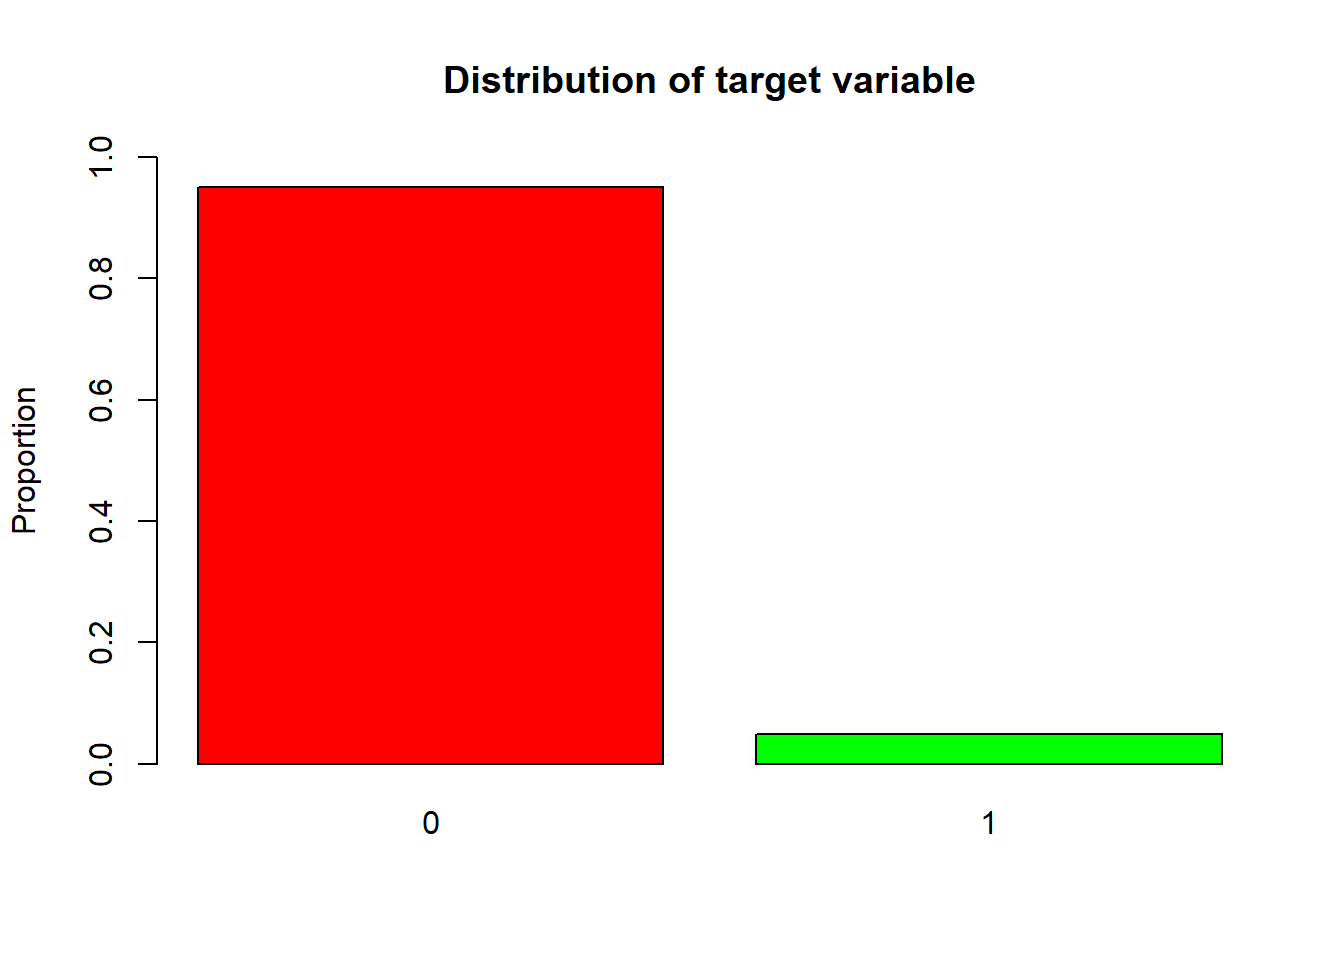
\includegraphics{Final_Project_files/figure-latex/unnamed-chunk-11-1.pdf}

\begin{Shaded}
\begin{Highlighting}[]
\CommentTok{\# Density plot for age}
\FunctionTok{plot}\NormalTok{(}\FunctionTok{density}\NormalTok{(stroke}\SpecialCharTok{$}\NormalTok{age), }\AttributeTok{main =} \StringTok{"Density Plot of Age"}\NormalTok{, }\AttributeTok{xlab =} \StringTok{"Age"}\NormalTok{, }\AttributeTok{col =} \StringTok{"blue"}\NormalTok{, }\AttributeTok{lwd =} \DecValTok{2}\NormalTok{)}

\CommentTok{\# Add a rug plot for individual data points}
\FunctionTok{rug}\NormalTok{(stroke}\SpecialCharTok{$}\NormalTok{age, }\AttributeTok{col =} \StringTok{"red"}\NormalTok{)}
\end{Highlighting}
\end{Shaded}

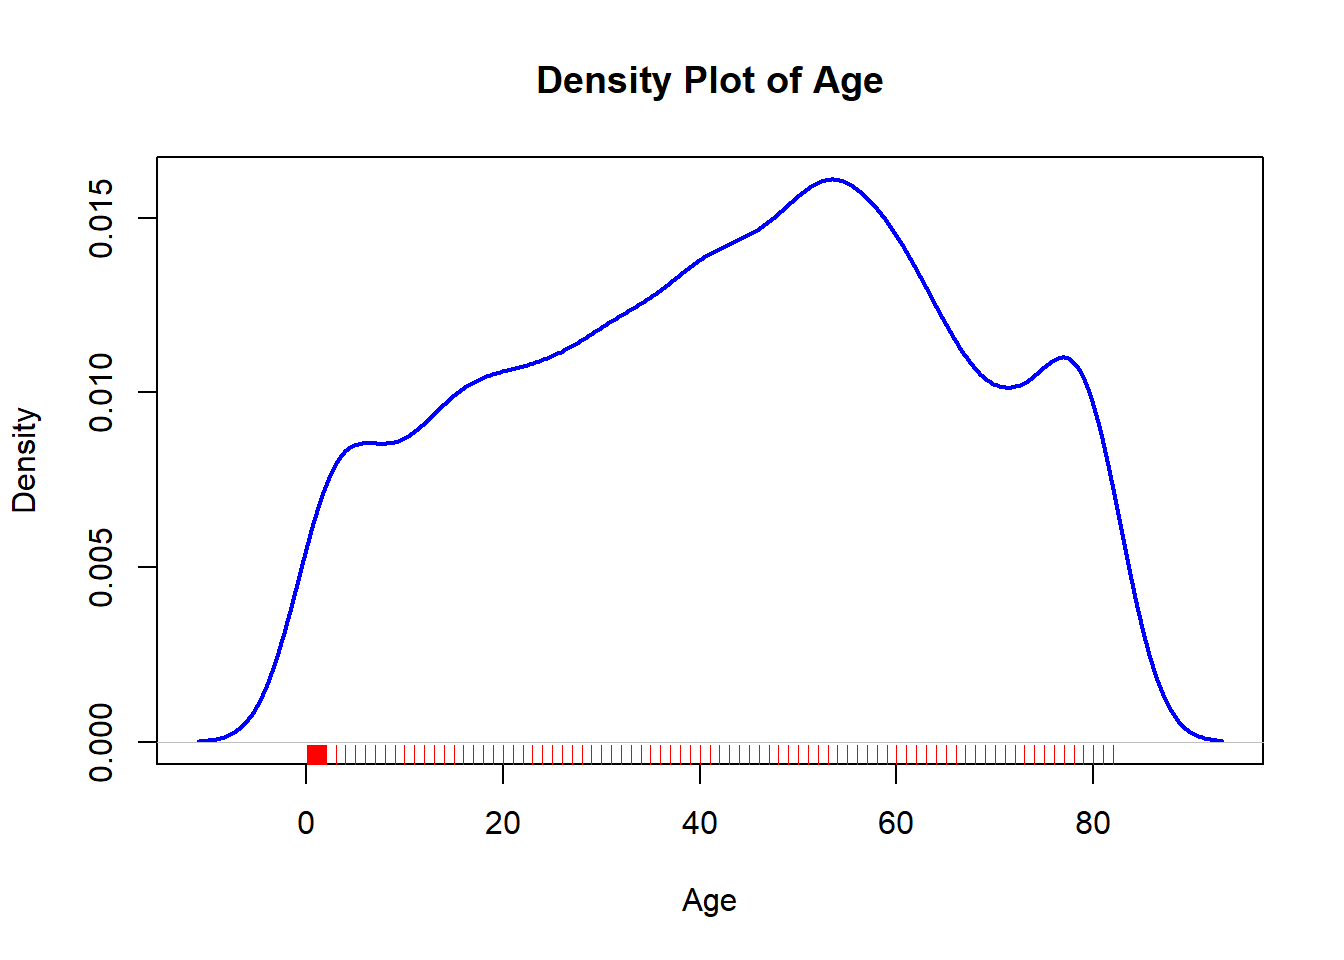
\includegraphics{Final_Project_files/figure-latex/unnamed-chunk-12-1.pdf}

\begin{Shaded}
\begin{Highlighting}[]
\CommentTok{\# Density plot for age}
\FunctionTok{plot}\NormalTok{(}\FunctionTok{density}\NormalTok{(stroke}\SpecialCharTok{$}\NormalTok{avg\_glucose\_level), }\AttributeTok{main =} \StringTok{"Density Plot of Avarage Glucose level"}\NormalTok{, }\AttributeTok{xlab =} \StringTok{"avg\_glucose\_level"}\NormalTok{, }\AttributeTok{col =} \StringTok{"blue"}\NormalTok{, }\AttributeTok{lwd =} \DecValTok{2}\NormalTok{)}

\CommentTok{\# Add a rug plot for individual data points}
\FunctionTok{rug}\NormalTok{(stroke}\SpecialCharTok{$}\NormalTok{avg\_glucose\_level, }\AttributeTok{col =} \StringTok{"red"}\NormalTok{)}
\end{Highlighting}
\end{Shaded}

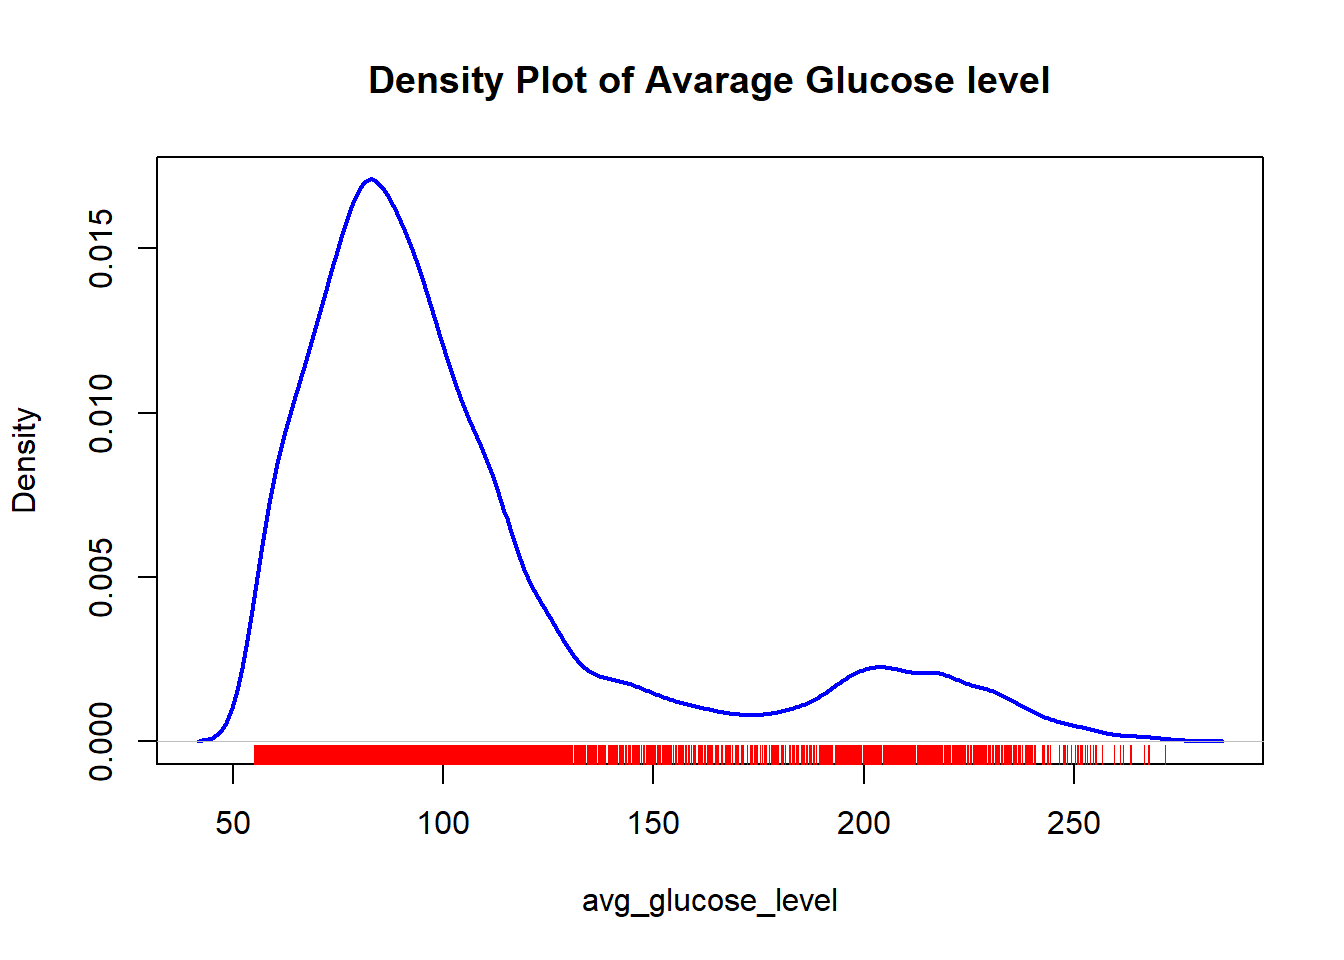
\includegraphics{Final_Project_files/figure-latex/unnamed-chunk-13-1.pdf}

\begin{Shaded}
\begin{Highlighting}[]
\CommentTok{\# Density plot for age}
\FunctionTok{plot}\NormalTok{(}\FunctionTok{density}\NormalTok{(stroke}\SpecialCharTok{$}\NormalTok{bmi), }\AttributeTok{main =} \StringTok{"Density Plot of BMI"}\NormalTok{, }\AttributeTok{xlab =} \StringTok{"BMI"}\NormalTok{, }\AttributeTok{col =} \StringTok{"blue"}\NormalTok{, }\AttributeTok{lwd =} \DecValTok{2}\NormalTok{)}

\CommentTok{\# Add a rug plot for individual data points}
\FunctionTok{rug}\NormalTok{(stroke}\SpecialCharTok{$}\NormalTok{bmi, }\AttributeTok{col =} \StringTok{"red"}\NormalTok{)}
\end{Highlighting}
\end{Shaded}

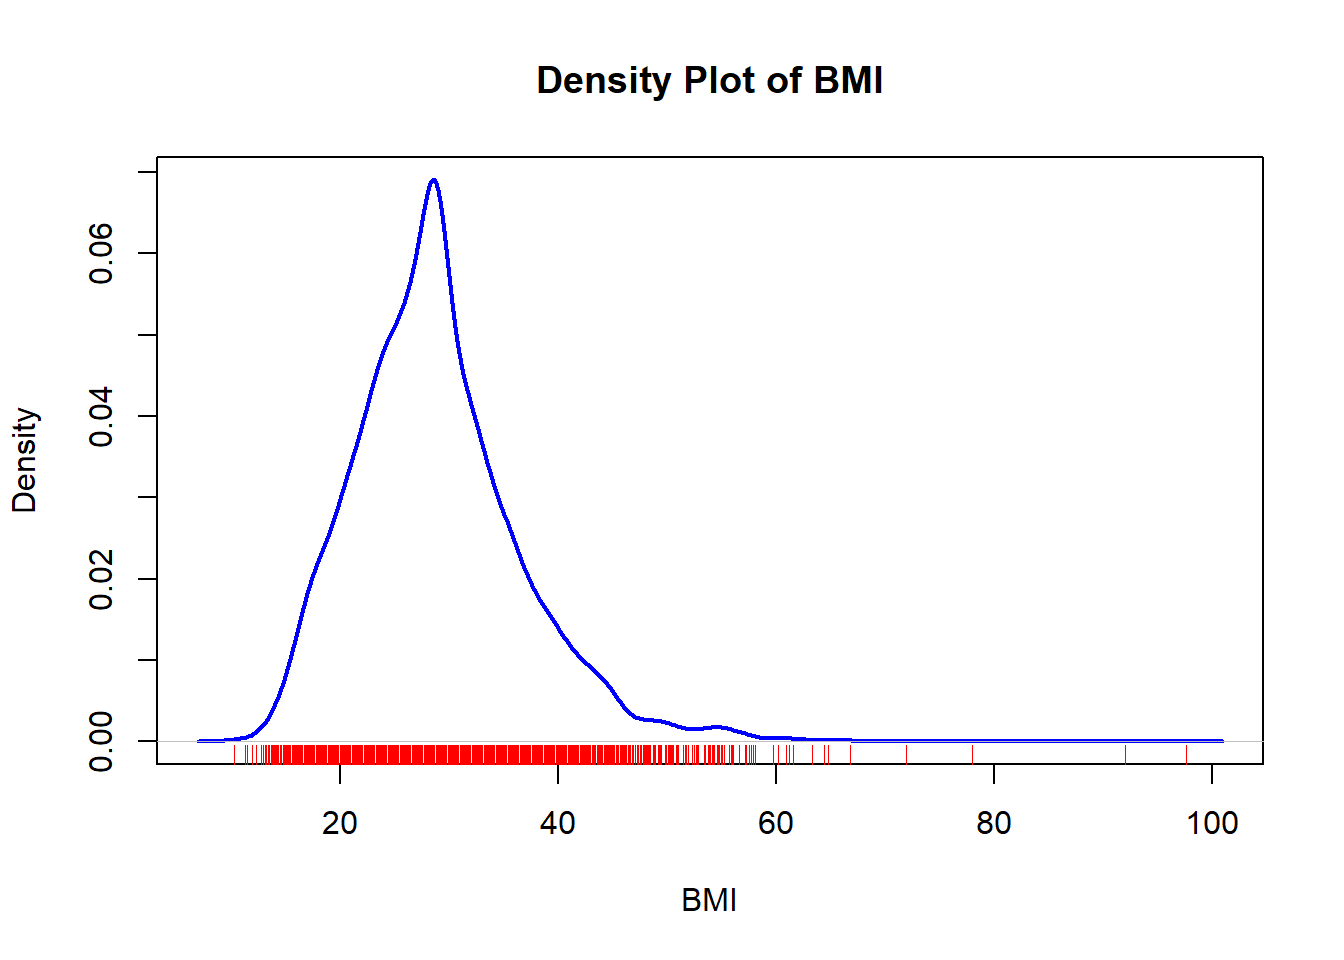
\includegraphics{Final_Project_files/figure-latex/unnamed-chunk-14-1.pdf}

\begin{Shaded}
\begin{Highlighting}[]
\CommentTok{\# Boxplot for age}
\FunctionTok{boxplot}\NormalTok{(stroke}\SpecialCharTok{$}\NormalTok{age, }\AttributeTok{main =} \StringTok{"Boxplot of Age"}\NormalTok{, }\AttributeTok{col =} \StringTok{"lightgreen"}\NormalTok{, }\AttributeTok{border =} \StringTok{"black"}\NormalTok{)}
\end{Highlighting}
\end{Shaded}

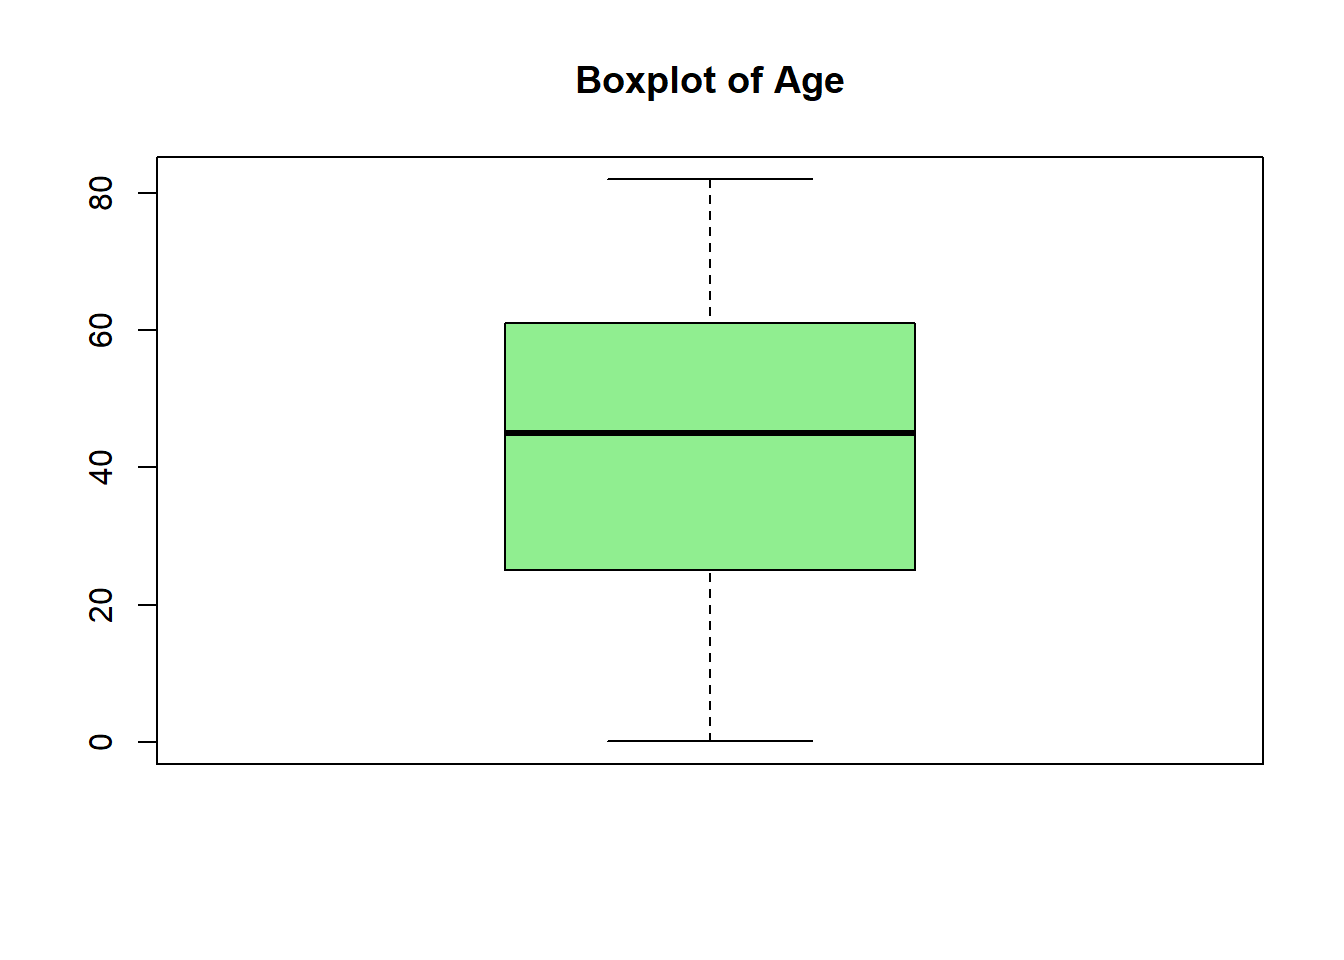
\includegraphics{Final_Project_files/figure-latex/unnamed-chunk-15-1.pdf}

\begin{Shaded}
\begin{Highlighting}[]
\CommentTok{\# Boxplot for avg\_glucose\_level}
\FunctionTok{boxplot}\NormalTok{(stroke}\SpecialCharTok{$}\NormalTok{avg\_glucose\_level, }\AttributeTok{main =} \StringTok{"Boxplot of Avg Glucose Level"}\NormalTok{, }\AttributeTok{col =} \StringTok{"lightblue"}\NormalTok{, }\AttributeTok{border =} \StringTok{"black"}\NormalTok{)}
\end{Highlighting}
\end{Shaded}

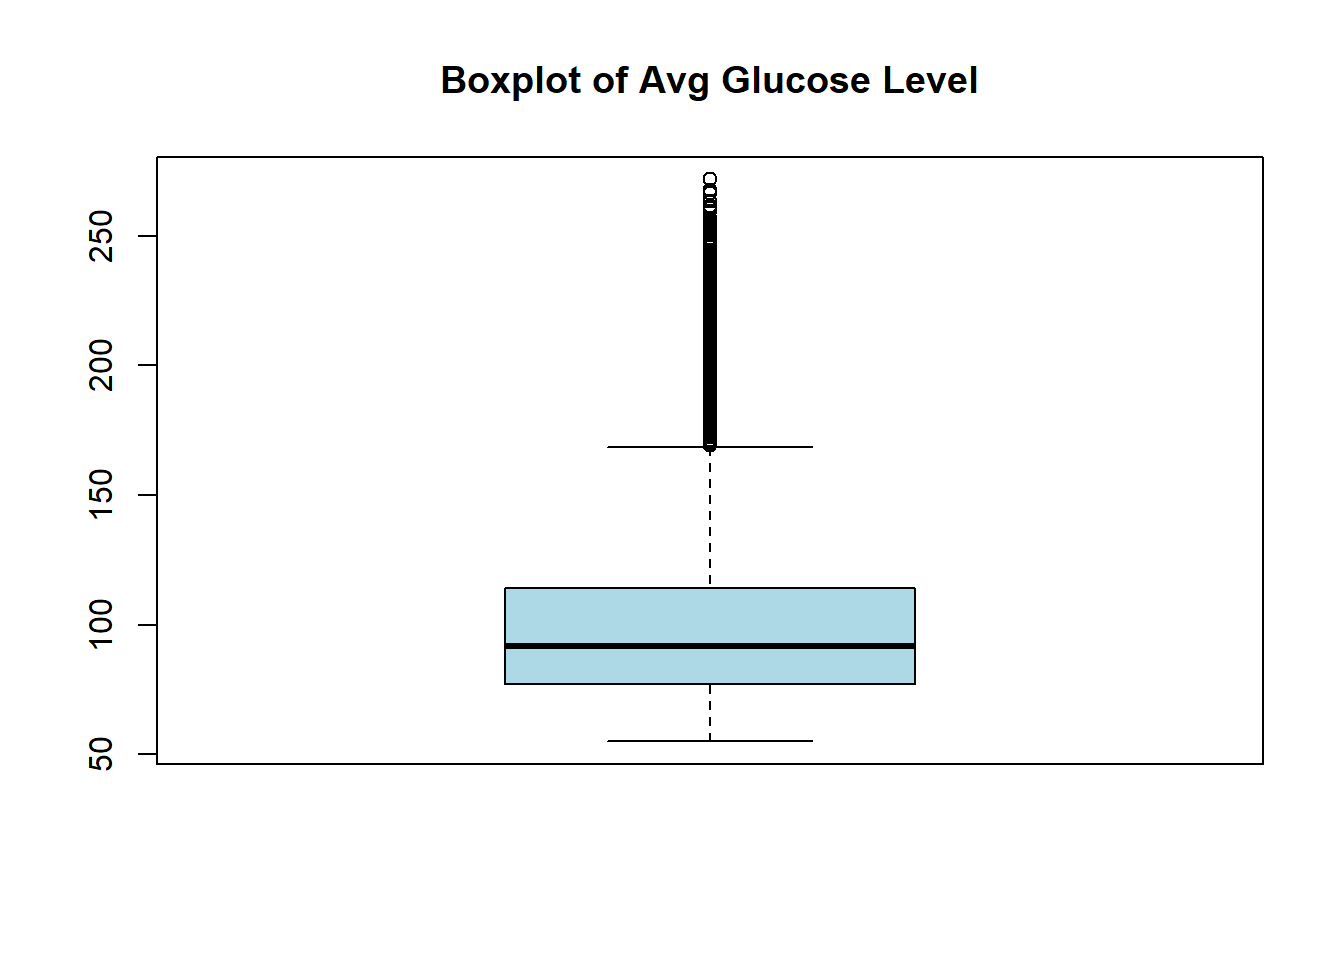
\includegraphics{Final_Project_files/figure-latex/unnamed-chunk-16-1.pdf}

\begin{Shaded}
\begin{Highlighting}[]
\CommentTok{\# Boxplot for bmi}
\FunctionTok{boxplot}\NormalTok{(stroke}\SpecialCharTok{$}\NormalTok{bmi, }\AttributeTok{main =} \StringTok{"Boxplot of BMI"}\NormalTok{, }\AttributeTok{col =} \StringTok{"lightcoral"}\NormalTok{, }\AttributeTok{border =} \StringTok{"black"}\NormalTok{)}
\end{Highlighting}
\end{Shaded}

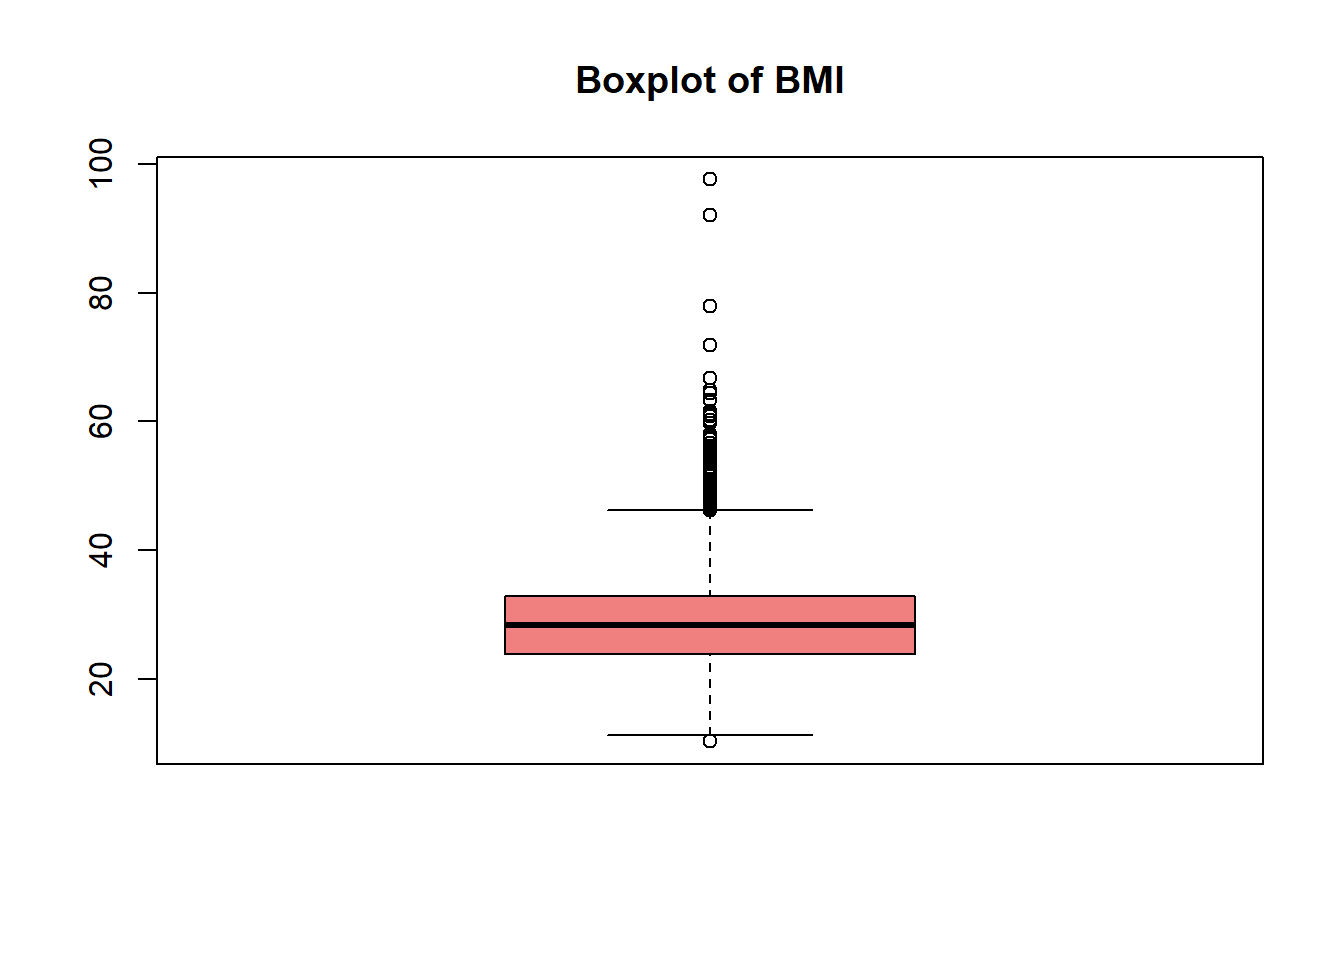
\includegraphics{Final_Project_files/figure-latex/unnamed-chunk-17-1.pdf}

\begin{Shaded}
\begin{Highlighting}[]
\CommentTok{\# Create a pie chart for gender}
\NormalTok{gender\_counts }\OtherTok{\textless{}{-}} \FunctionTok{table}\NormalTok{(stroke}\SpecialCharTok{$}\NormalTok{gender)}
\NormalTok{gender\_percentages }\OtherTok{\textless{}{-}} \FunctionTok{round}\NormalTok{(}\FunctionTok{prop.table}\NormalTok{(gender\_counts) }\SpecialCharTok{*} \DecValTok{100}\NormalTok{, }\DecValTok{1}\NormalTok{)}
\FunctionTok{pie}\NormalTok{(gender\_counts, }\AttributeTok{labels =} \FunctionTok{paste}\NormalTok{(}\FunctionTok{names}\NormalTok{(gender\_counts), }\StringTok{"}\SpecialCharTok{\textbackslash{}n}\StringTok{"}\NormalTok{, gender\_percentages, }\StringTok{"\%"}\NormalTok{), }\AttributeTok{main =} \StringTok{"Distribution of Gender"}\NormalTok{, }\AttributeTok{col =} \FunctionTok{rainbow}\NormalTok{(}\FunctionTok{length}\NormalTok{(gender\_counts)))}
\end{Highlighting}
\end{Shaded}

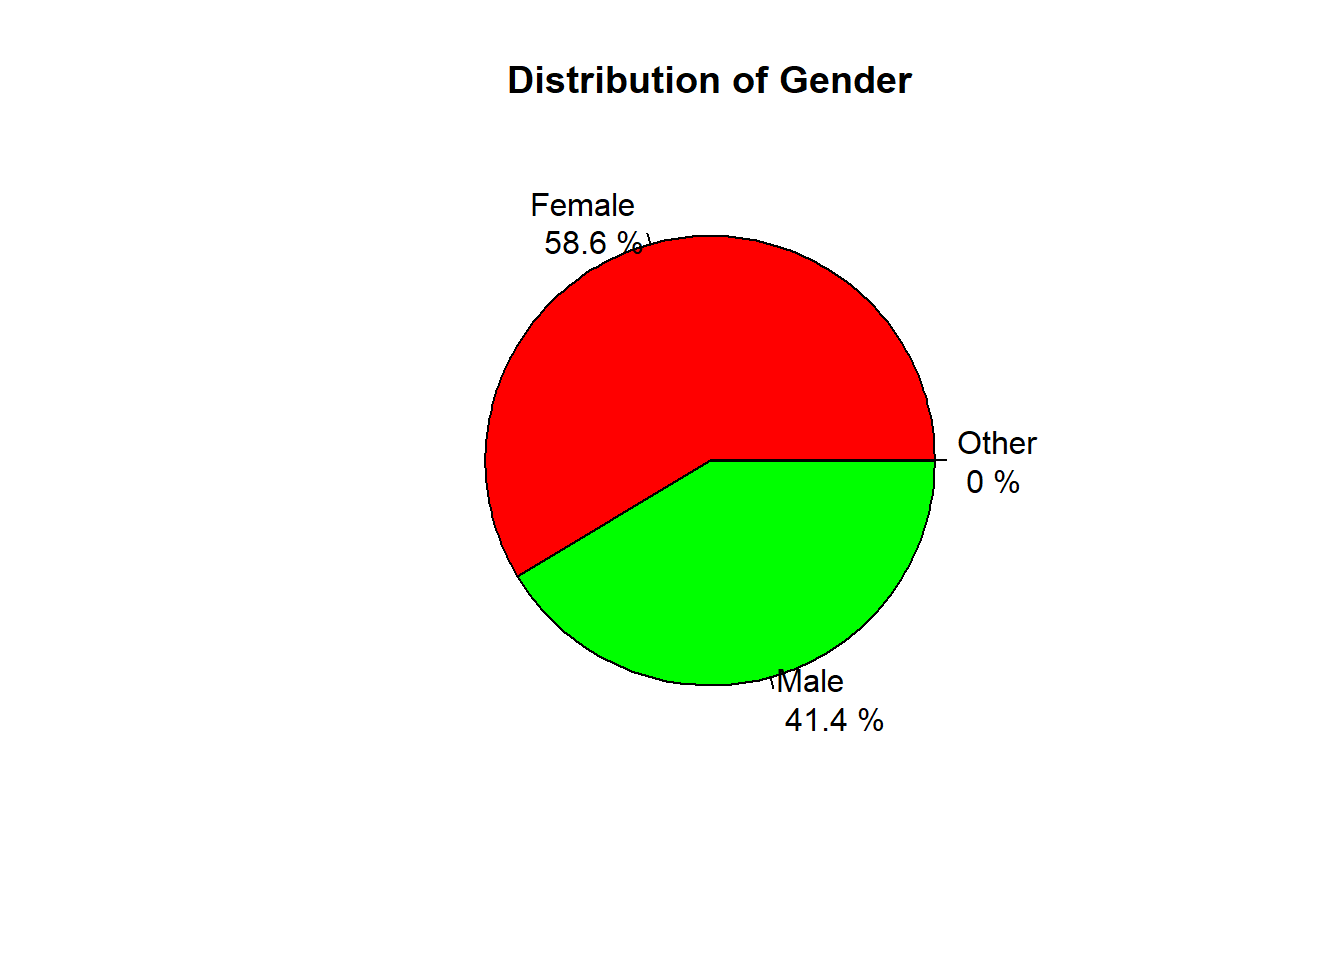
\includegraphics{Final_Project_files/figure-latex/unnamed-chunk-18-1.pdf}

\begin{Shaded}
\begin{Highlighting}[]
\CommentTok{\# Create a pie chart for ever\_married}
\NormalTok{married\_counts }\OtherTok{\textless{}{-}} \FunctionTok{table}\NormalTok{(stroke}\SpecialCharTok{$}\NormalTok{ever\_married)}
\NormalTok{married\_percentages }\OtherTok{\textless{}{-}} \FunctionTok{round}\NormalTok{(}\FunctionTok{prop.table}\NormalTok{(married\_counts) }\SpecialCharTok{*} \DecValTok{100}\NormalTok{, }\DecValTok{1}\NormalTok{)}
\FunctionTok{pie}\NormalTok{(married\_counts, }\AttributeTok{labels =} \FunctionTok{paste}\NormalTok{(}\FunctionTok{names}\NormalTok{(married\_counts), }\StringTok{"}\SpecialCharTok{\textbackslash{}n}\StringTok{"}\NormalTok{, married\_percentages, }\StringTok{"\%"}\NormalTok{), }\AttributeTok{main =} \StringTok{"Distribution of Marital Status"}\NormalTok{, }\AttributeTok{col =} \FunctionTok{rainbow}\NormalTok{(}\FunctionTok{length}\NormalTok{(married\_counts)))}
\end{Highlighting}
\end{Shaded}

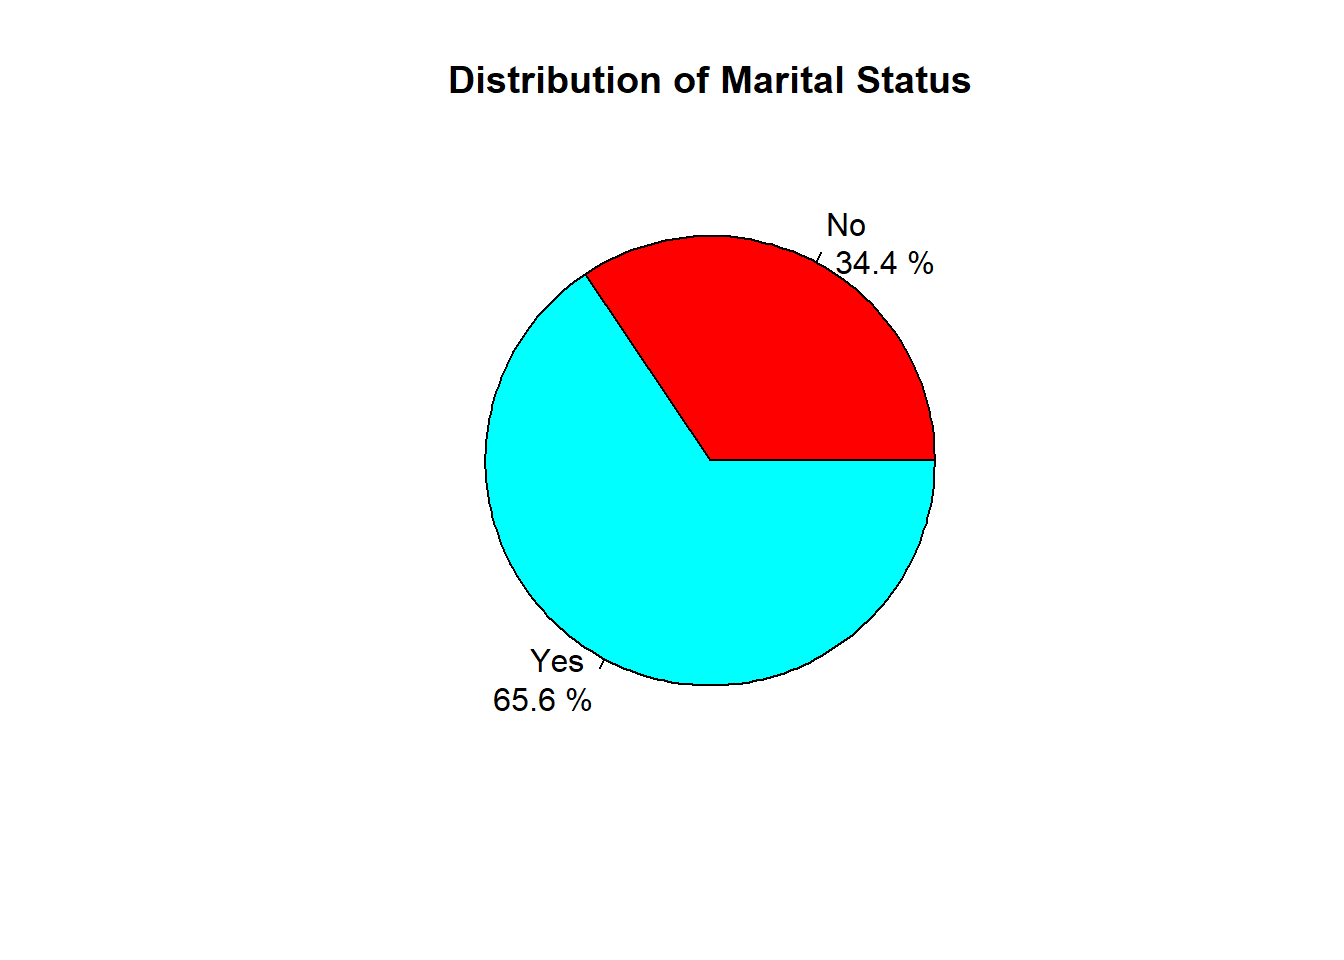
\includegraphics{Final_Project_files/figure-latex/unnamed-chunk-18-2.pdf}

\begin{Shaded}
\begin{Highlighting}[]
\CommentTok{\# Create a pie chart for work\_type}
\NormalTok{work\_counts }\OtherTok{\textless{}{-}} \FunctionTok{table}\NormalTok{(stroke}\SpecialCharTok{$}\NormalTok{work\_type)}
\NormalTok{work\_percentages }\OtherTok{\textless{}{-}} \FunctionTok{round}\NormalTok{(}\FunctionTok{prop.table}\NormalTok{(work\_counts) }\SpecialCharTok{*} \DecValTok{100}\NormalTok{, }\DecValTok{1}\NormalTok{)}
\FunctionTok{pie}\NormalTok{(work\_counts, }\AttributeTok{labels =} \FunctionTok{paste}\NormalTok{(}\FunctionTok{names}\NormalTok{(work\_counts), }\StringTok{"}\SpecialCharTok{\textbackslash{}n}\StringTok{"}\NormalTok{, work\_percentages, }\StringTok{"\%"}\NormalTok{), }\AttributeTok{main =} \StringTok{"Distribution of Work Type"}\NormalTok{, }\AttributeTok{col =} \FunctionTok{rainbow}\NormalTok{(}\FunctionTok{length}\NormalTok{(work\_counts)))}
\end{Highlighting}
\end{Shaded}

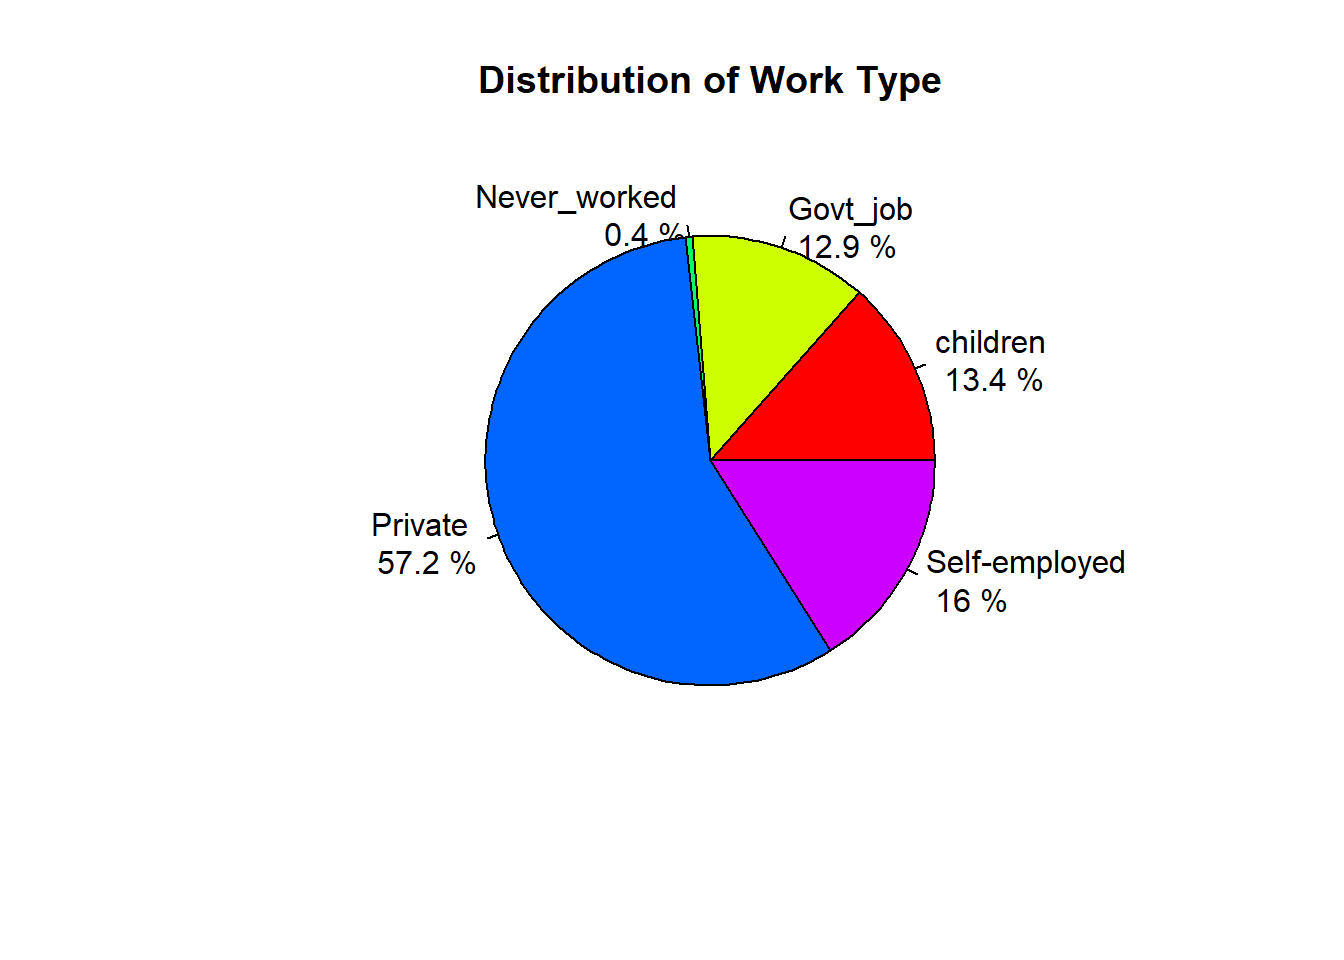
\includegraphics{Final_Project_files/figure-latex/unnamed-chunk-18-3.pdf}

\begin{Shaded}
\begin{Highlighting}[]
\CommentTok{\# Create a pie chart for Residence\_type}
\NormalTok{residence\_counts }\OtherTok{\textless{}{-}} \FunctionTok{table}\NormalTok{(stroke}\SpecialCharTok{$}\NormalTok{Residence\_type)}
\NormalTok{residence\_percentages }\OtherTok{\textless{}{-}} \FunctionTok{round}\NormalTok{(}\FunctionTok{prop.table}\NormalTok{(residence\_counts) }\SpecialCharTok{*} \DecValTok{100}\NormalTok{, }\DecValTok{1}\NormalTok{)}
\FunctionTok{pie}\NormalTok{(residence\_counts, }\AttributeTok{labels =} \FunctionTok{paste}\NormalTok{(}\FunctionTok{names}\NormalTok{(residence\_counts), }\StringTok{"}\SpecialCharTok{\textbackslash{}n}\StringTok{"}\NormalTok{, residence\_percentages, }\StringTok{"\%"}\NormalTok{), }\AttributeTok{main =} \StringTok{"Distribution of Residence Type"}\NormalTok{, }\AttributeTok{col =} \FunctionTok{rainbow}\NormalTok{(}\FunctionTok{length}\NormalTok{(residence\_counts)))}
\end{Highlighting}
\end{Shaded}

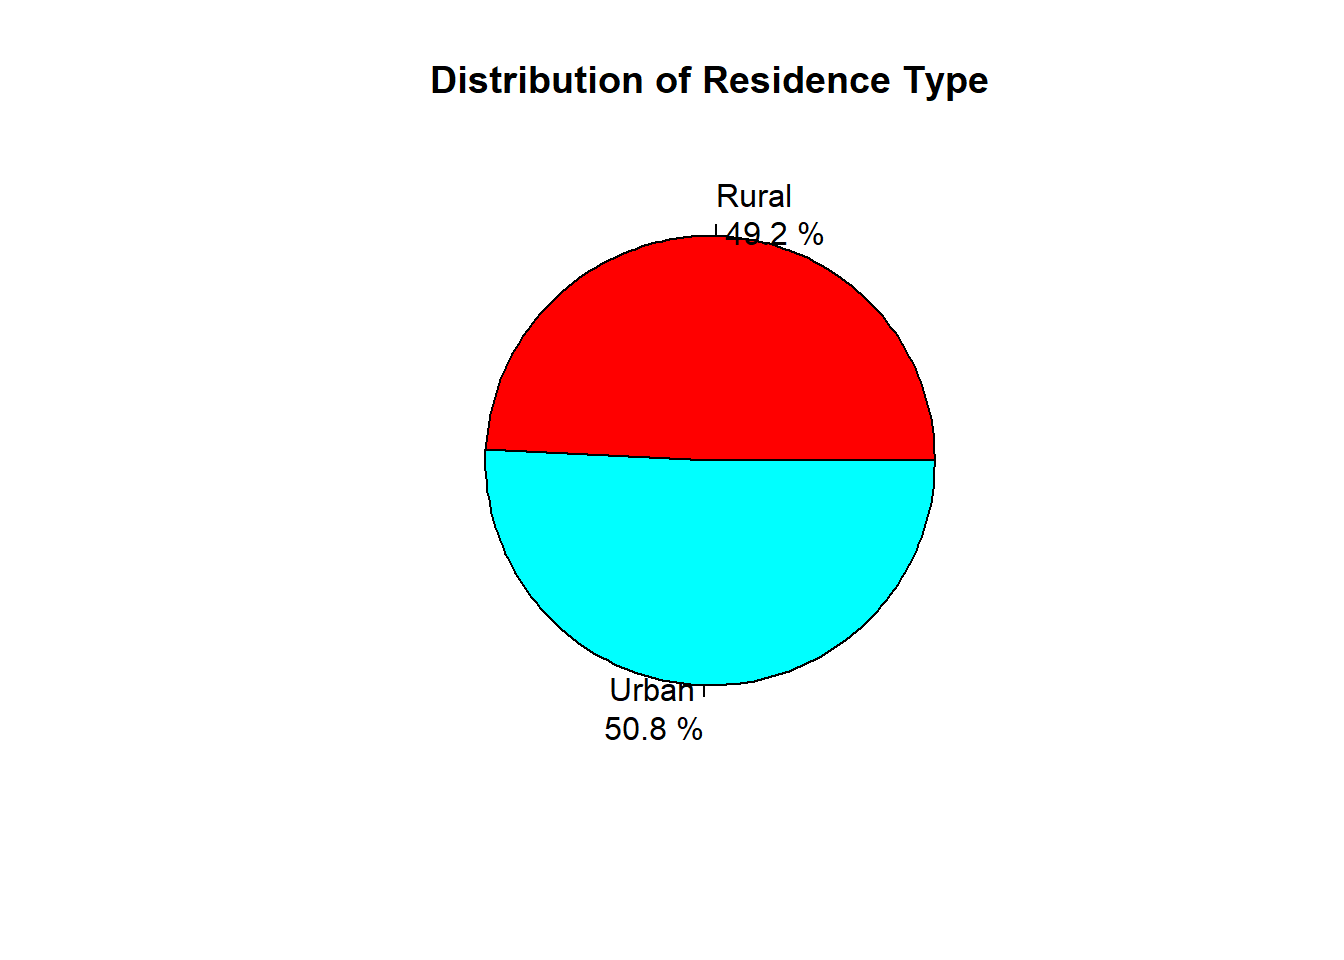
\includegraphics{Final_Project_files/figure-latex/unnamed-chunk-18-4.pdf}

\begin{Shaded}
\begin{Highlighting}[]
\CommentTok{\# Create a pie chart for Residence\_type}
\NormalTok{smoke\_counts }\OtherTok{\textless{}{-}} \FunctionTok{table}\NormalTok{(stroke}\SpecialCharTok{$}\NormalTok{smoking\_status)}
\NormalTok{smoke\_percentages }\OtherTok{\textless{}{-}} \FunctionTok{round}\NormalTok{(}\FunctionTok{prop.table}\NormalTok{(smoke\_counts) }\SpecialCharTok{*} \DecValTok{100}\NormalTok{, }\DecValTok{1}\NormalTok{)}
\FunctionTok{pie}\NormalTok{(smoke\_counts, }\AttributeTok{labels =} \FunctionTok{paste}\NormalTok{(}\FunctionTok{names}\NormalTok{(smoke\_counts), }\StringTok{"}\SpecialCharTok{\textbackslash{}n}\StringTok{"}\NormalTok{, smoke\_percentages, }\StringTok{"\%"}\NormalTok{), }\AttributeTok{main =} \StringTok{"Distribution of Smoking status"}\NormalTok{, }\AttributeTok{col =} \FunctionTok{rainbow}\NormalTok{(}\FunctionTok{length}\NormalTok{(residence\_counts)))}
\end{Highlighting}
\end{Shaded}

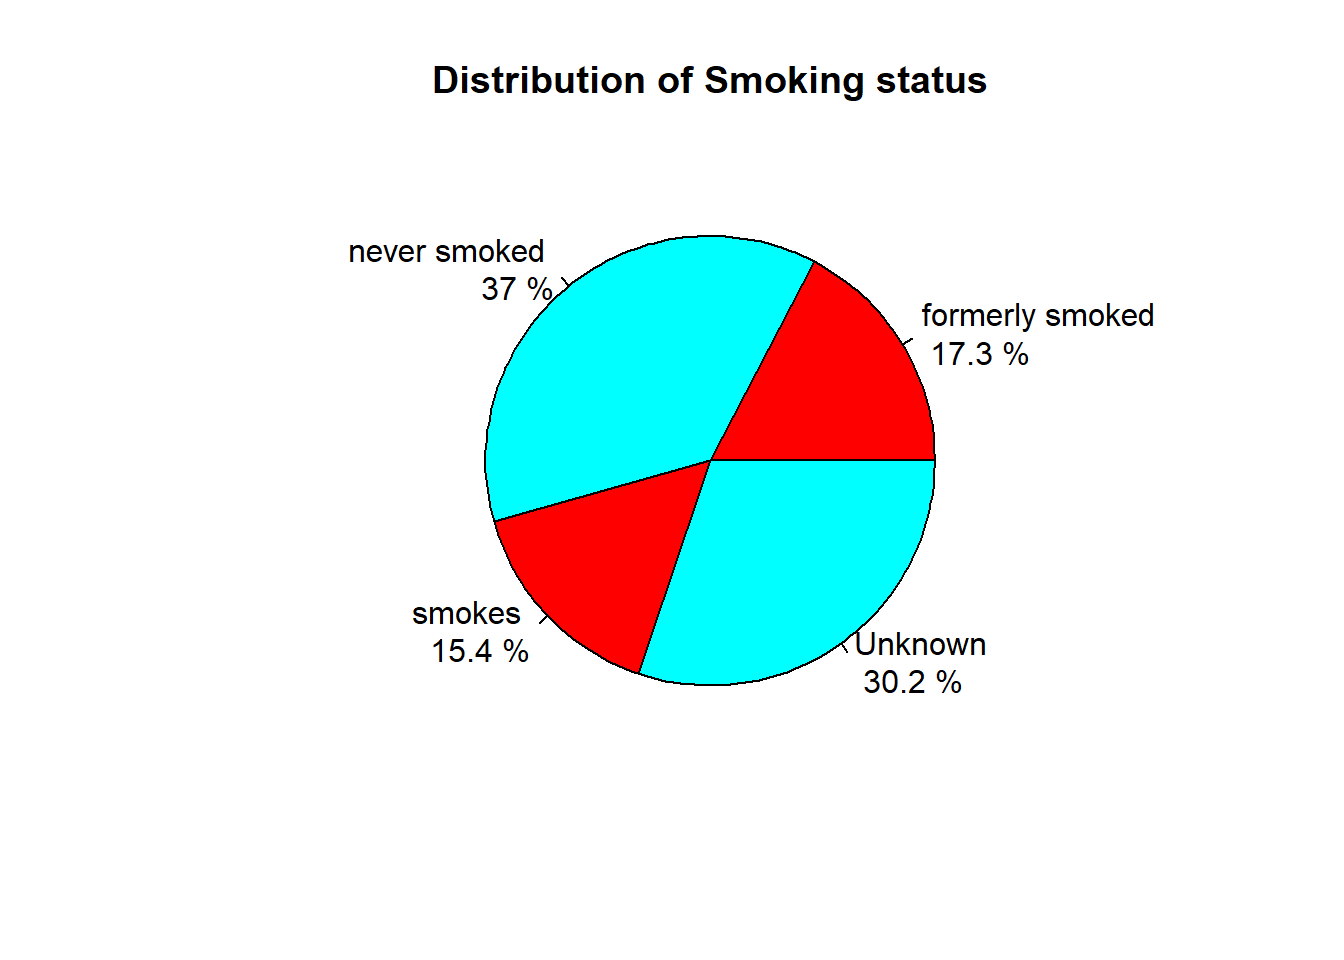
\includegraphics{Final_Project_files/figure-latex/unnamed-chunk-18-5.pdf}

\begin{Shaded}
\begin{Highlighting}[]
\CommentTok{\# Boxplot for age with respect to stroke}
\FunctionTok{boxplot}\NormalTok{(age }\SpecialCharTok{\textasciitilde{}}\NormalTok{ stroke, }\AttributeTok{data =}\NormalTok{ stroke, }\AttributeTok{main =} \StringTok{"Age Distribution by Stroke"}\NormalTok{, }\AttributeTok{xlab =} \StringTok{"Stroke"}\NormalTok{, }\AttributeTok{ylab =} \StringTok{"Age"}\NormalTok{, }\AttributeTok{col =} \FunctionTok{c}\NormalTok{(}\StringTok{"lightgreen"}\NormalTok{, }\StringTok{"lightcoral"}\NormalTok{))}
\end{Highlighting}
\end{Shaded}

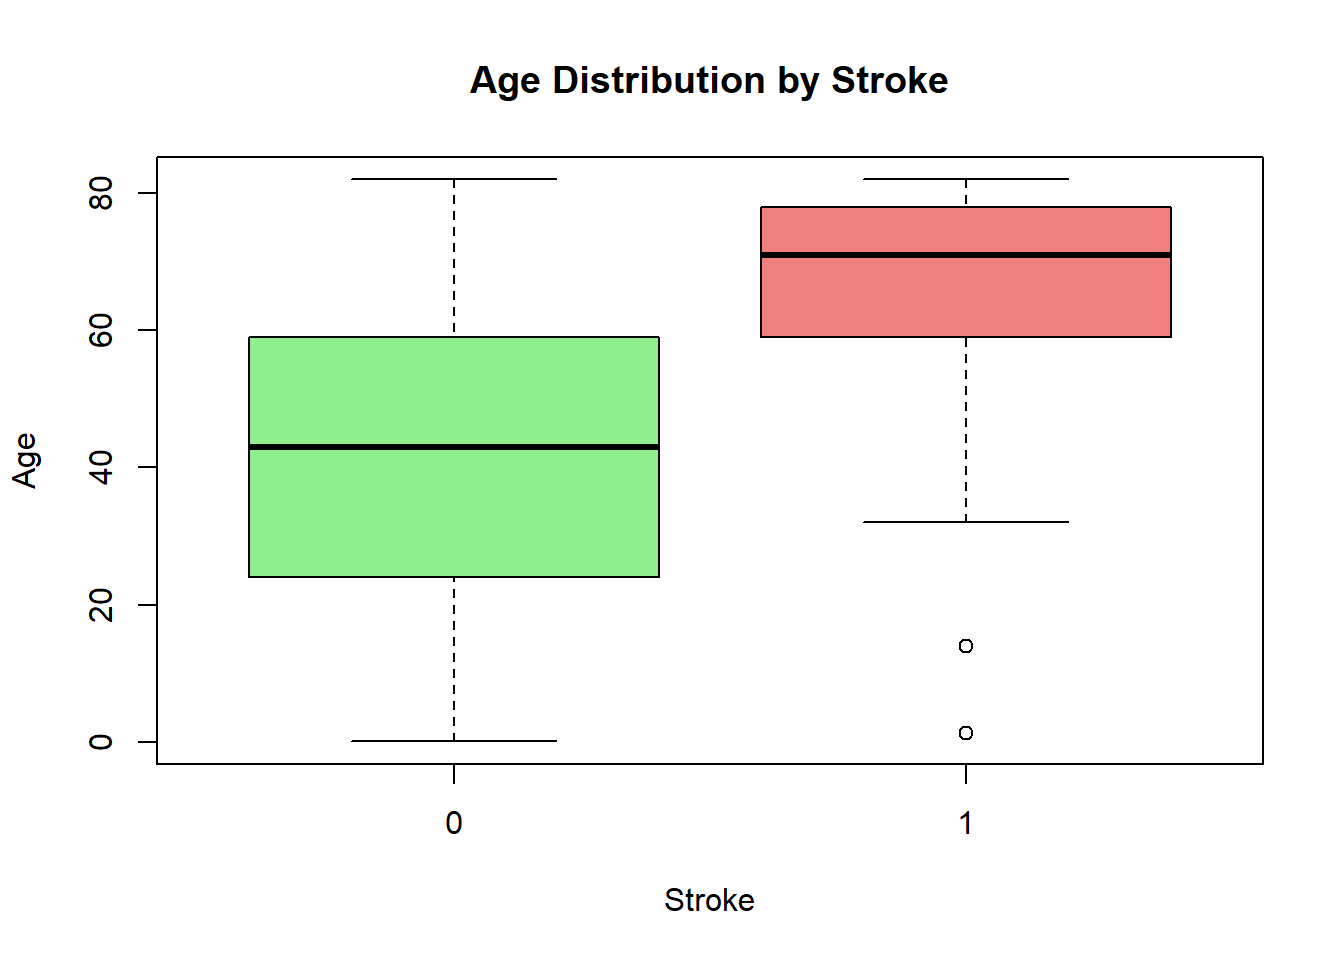
\includegraphics{Final_Project_files/figure-latex/unnamed-chunk-19-1.pdf}

\begin{Shaded}
\begin{Highlighting}[]
\CommentTok{\# Boxplot for avg\_glucose\_level with respect to stroke}
\FunctionTok{boxplot}\NormalTok{(avg\_glucose\_level }\SpecialCharTok{\textasciitilde{}}\NormalTok{ stroke, }\AttributeTok{data =}\NormalTok{ stroke, }\AttributeTok{main =} \StringTok{"Avg Glucose Level by Stroke"}\NormalTok{, }\AttributeTok{xlab =} \StringTok{"Stroke"}\NormalTok{, }\AttributeTok{ylab =} \StringTok{"Avg Glucose Level"}\NormalTok{, }\AttributeTok{col =} \FunctionTok{c}\NormalTok{(}\StringTok{"lightgreen"}\NormalTok{, }\StringTok{"lightcoral"}\NormalTok{))}
\end{Highlighting}
\end{Shaded}

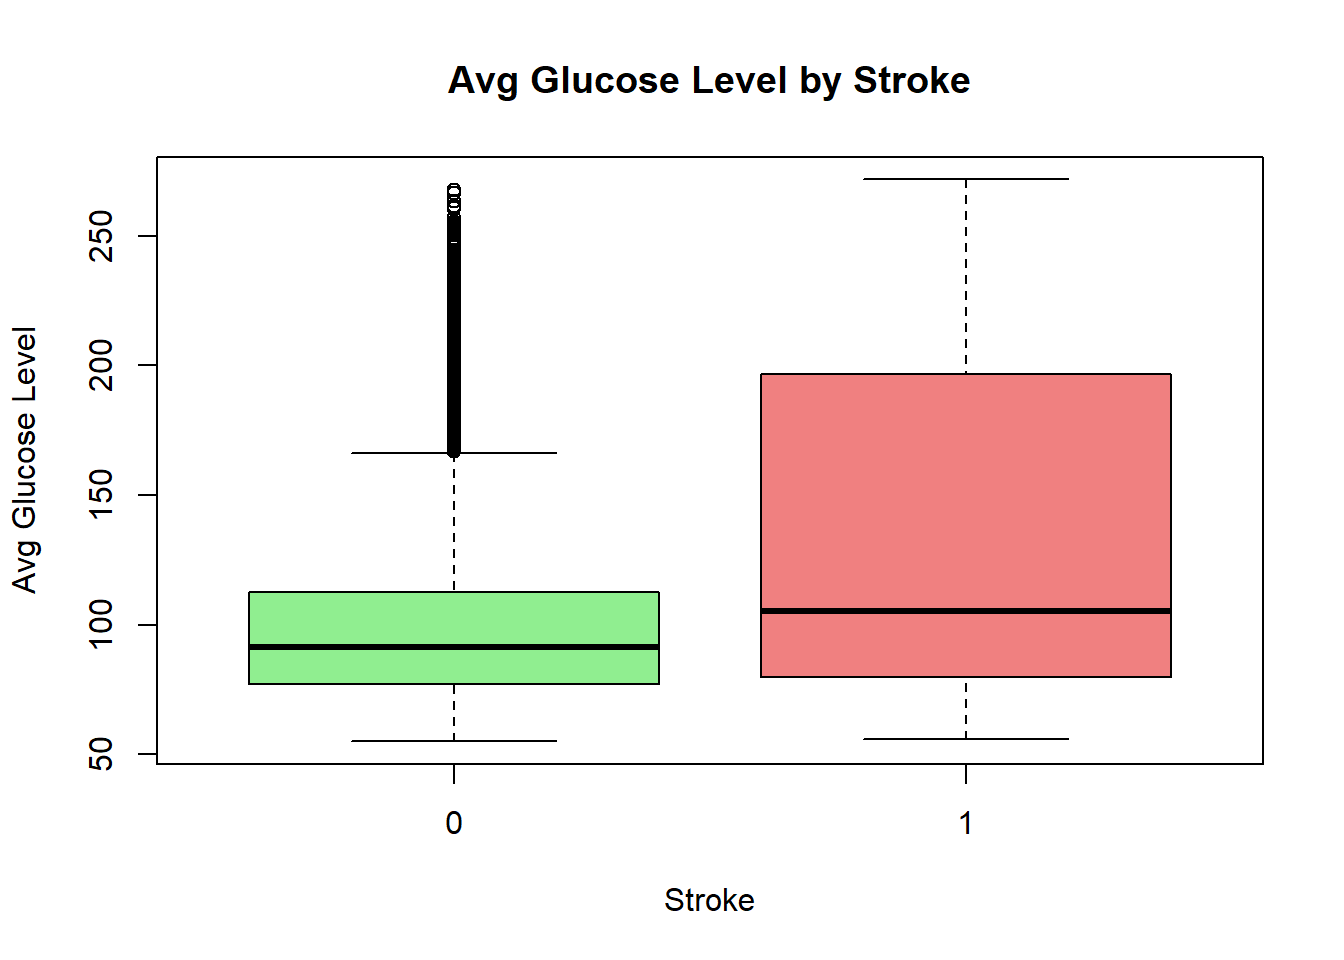
\includegraphics{Final_Project_files/figure-latex/unnamed-chunk-19-2.pdf}

\begin{Shaded}
\begin{Highlighting}[]
\CommentTok{\# Boxplot for bmi with respect to stroke}
\FunctionTok{boxplot}\NormalTok{(bmi }\SpecialCharTok{\textasciitilde{}}\NormalTok{ stroke, }\AttributeTok{data =}\NormalTok{ stroke, }\AttributeTok{main =} \StringTok{"BMI Distribution by Stroke"}\NormalTok{, }\AttributeTok{xlab =} \StringTok{"Stroke"}\NormalTok{, }\AttributeTok{ylab =} \StringTok{"BMI"}\NormalTok{, }\AttributeTok{col =} \FunctionTok{c}\NormalTok{(}\StringTok{"lightgreen"}\NormalTok{, }\StringTok{"lightcoral"}\NormalTok{))}
\end{Highlighting}
\end{Shaded}

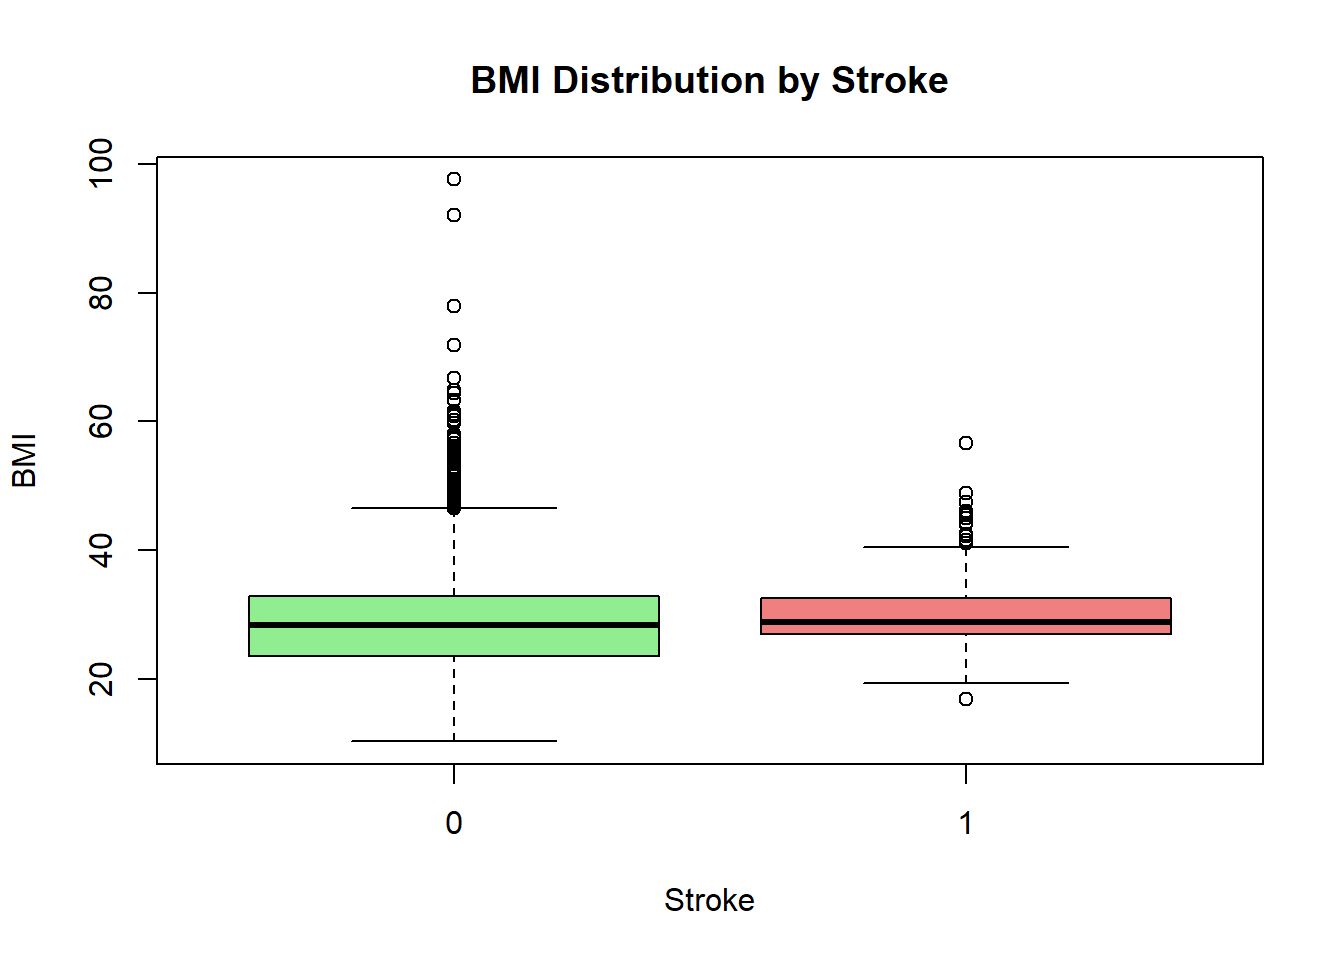
\includegraphics{Final_Project_files/figure-latex/unnamed-chunk-19-3.pdf}

\begin{Shaded}
\begin{Highlighting}[]
\CommentTok{\# Function to calculate percentages and create bar plots with different colors}
\NormalTok{plot\_categorical\_variable }\OtherTok{\textless{}{-}} \ControlFlowTok{function}\NormalTok{(variable, title, colors) \{}
\NormalTok{  percentages }\OtherTok{\textless{}{-}} \FunctionTok{prop.table}\NormalTok{(}\FunctionTok{table}\NormalTok{(stroke[[variable]], stroke}\SpecialCharTok{$}\NormalTok{stroke), }\AttributeTok{margin =} \DecValTok{2}\NormalTok{) }\SpecialCharTok{*} \DecValTok{100}
  \FunctionTok{ggplot}\NormalTok{(stroke, }\FunctionTok{aes}\NormalTok{(}\AttributeTok{x =} \FunctionTok{get}\NormalTok{(variable), }\AttributeTok{fill =} \FunctionTok{as.factor}\NormalTok{(stroke))) }\SpecialCharTok{+}
    \FunctionTok{geom\_bar}\NormalTok{(}\AttributeTok{position =} \StringTok{"fill"}\NormalTok{, }\AttributeTok{stat =} \StringTok{"count"}\NormalTok{) }\SpecialCharTok{+}
    \FunctionTok{scale\_y\_continuous}\NormalTok{(}\AttributeTok{labels =}\NormalTok{ scales}\SpecialCharTok{::}\FunctionTok{percent\_format}\NormalTok{(}\AttributeTok{scale =} \DecValTok{1}\NormalTok{)) }\SpecialCharTok{+}
    \FunctionTok{labs}\NormalTok{(}\AttributeTok{title =}\NormalTok{ title, }\AttributeTok{x =}\NormalTok{ variable, }\AttributeTok{y =} \StringTok{"Percentage"}\NormalTok{) }\SpecialCharTok{+}
    \FunctionTok{scale\_fill\_manual}\NormalTok{(}\AttributeTok{values =}\NormalTok{ colors) }\SpecialCharTok{+}
    \FunctionTok{theme\_minimal}\NormalTok{() }\SpecialCharTok{+}
    \FunctionTok{theme}\NormalTok{(}\AttributeTok{axis.text.x =} \FunctionTok{element\_text}\NormalTok{(}\AttributeTok{angle =} \DecValTok{45}\NormalTok{, }\AttributeTok{hjust =} \DecValTok{1}\NormalTok{))}
\NormalTok{\}}

\CommentTok{\# Create bar plots for each categorical variable with different colors}
\FunctionTok{plot\_categorical\_variable}\NormalTok{(}\StringTok{"gender"}\NormalTok{, }\StringTok{"Distribution of Gender by Stroke"}\NormalTok{, }\FunctionTok{c}\NormalTok{(}\StringTok{"skyblue"}\NormalTok{, }\StringTok{"pink"}\NormalTok{))}
\end{Highlighting}
\end{Shaded}

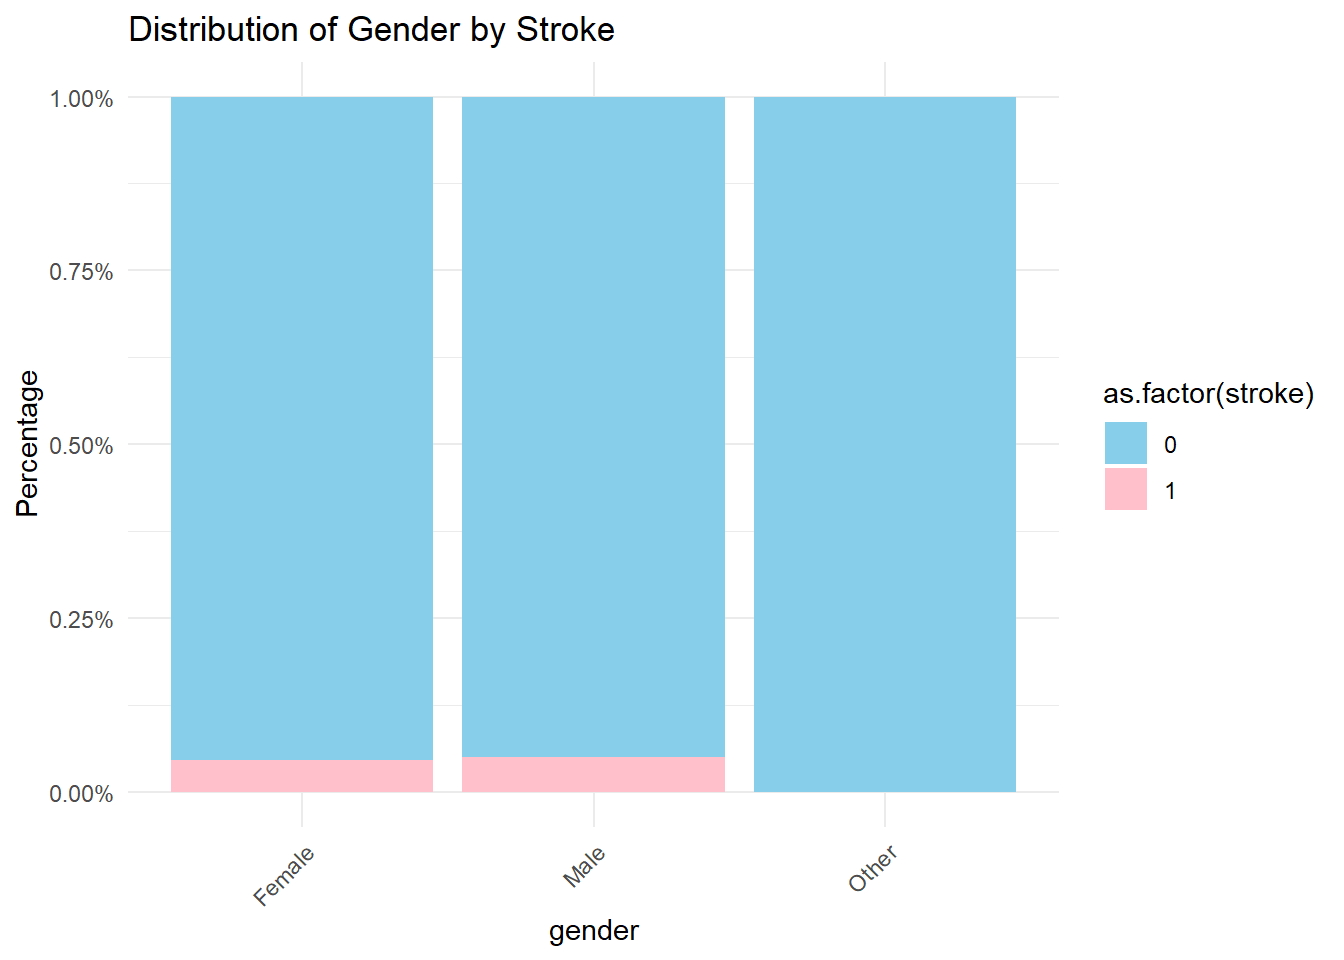
\includegraphics{Final_Project_files/figure-latex/unnamed-chunk-20-1.pdf}

\begin{Shaded}
\begin{Highlighting}[]
\FunctionTok{plot\_categorical\_variable}\NormalTok{(}\StringTok{"ever\_married"}\NormalTok{, }\StringTok{"Distribution of Marital Status by Stroke"}\NormalTok{, }\FunctionTok{c}\NormalTok{(}\StringTok{"lightgreen"}\NormalTok{, }\StringTok{"lightcoral"}\NormalTok{))}
\end{Highlighting}
\end{Shaded}

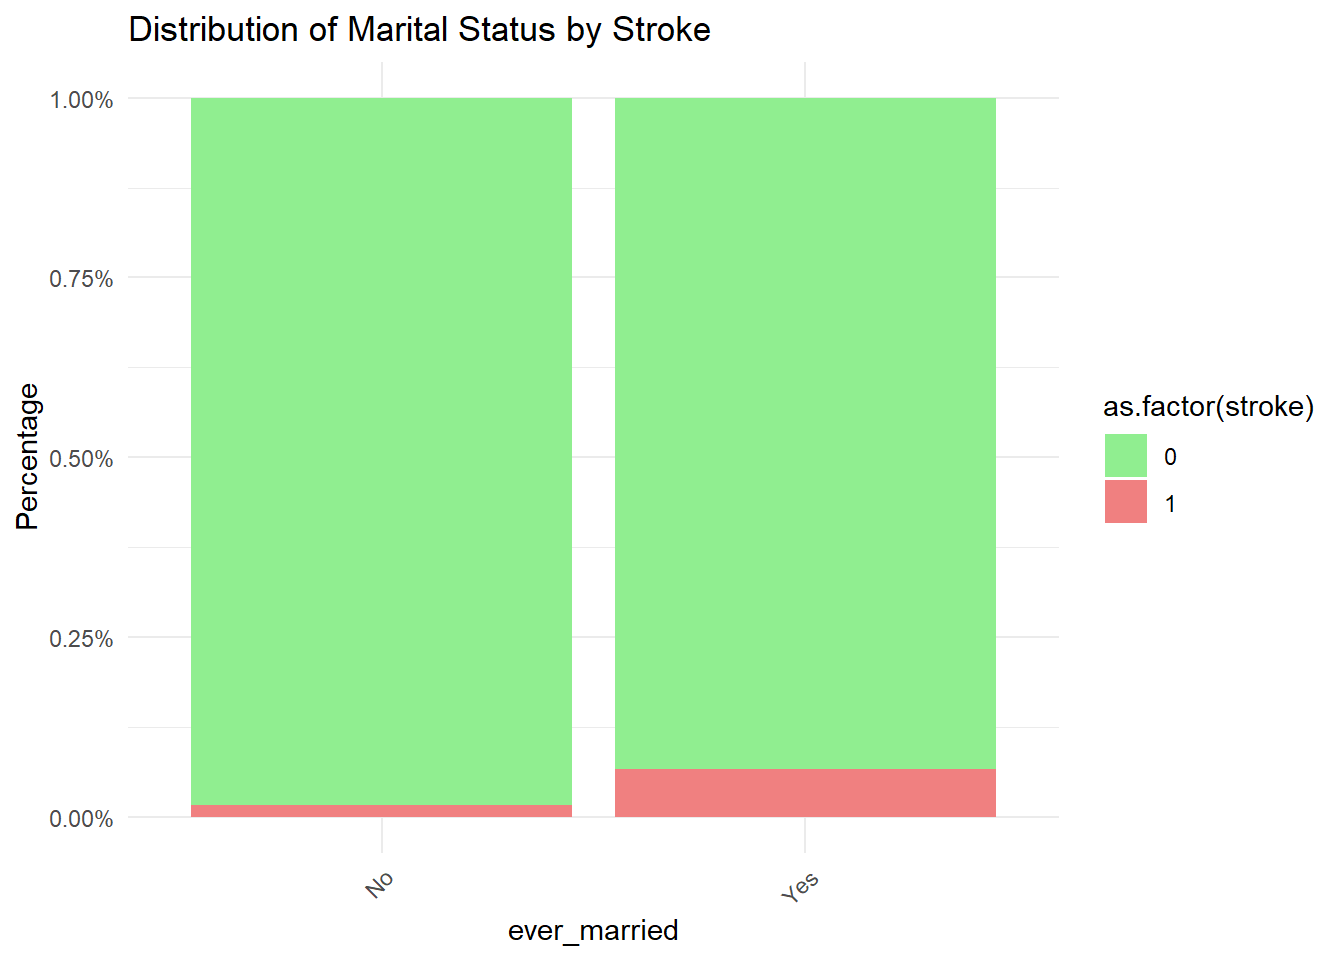
\includegraphics{Final_Project_files/figure-latex/unnamed-chunk-20-2.pdf}

\begin{Shaded}
\begin{Highlighting}[]
\FunctionTok{plot\_categorical\_variable}\NormalTok{(}\StringTok{"work\_type"}\NormalTok{, }\StringTok{"Distribution of Work Type by Stroke"}\NormalTok{, }\FunctionTok{c}\NormalTok{(}\StringTok{"lightblue"}\NormalTok{, }\StringTok{"salmon"}\NormalTok{))}
\end{Highlighting}
\end{Shaded}

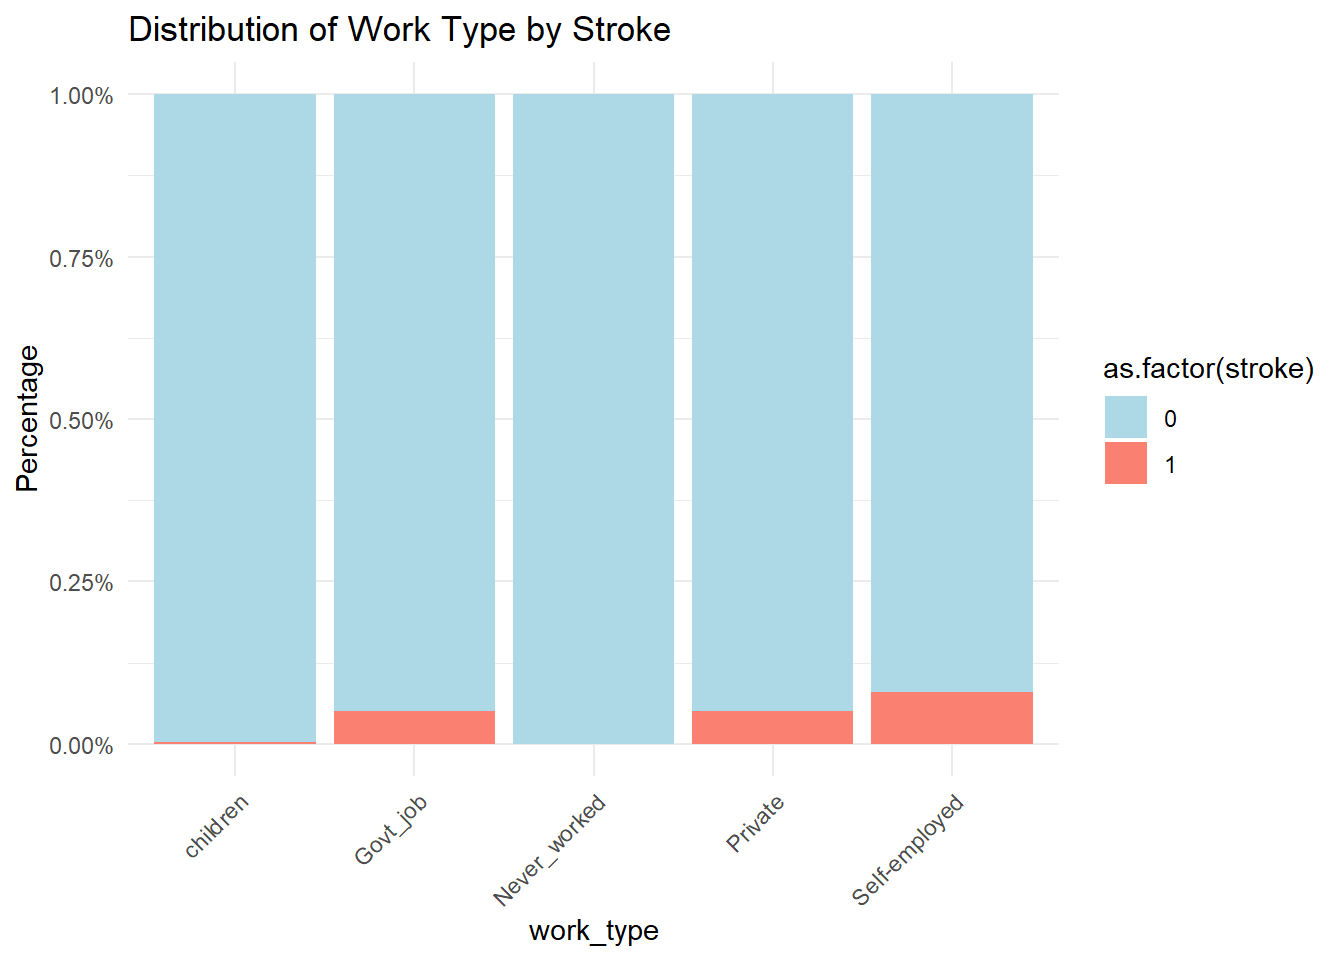
\includegraphics{Final_Project_files/figure-latex/unnamed-chunk-20-3.pdf}

\begin{Shaded}
\begin{Highlighting}[]
\FunctionTok{plot\_categorical\_variable}\NormalTok{(}\StringTok{"Residence\_type"}\NormalTok{, }\StringTok{"Distribution of Residence Type by Stroke"}\NormalTok{, }\FunctionTok{c}\NormalTok{(}\StringTok{"lightgoldenrod"}\NormalTok{, }\StringTok{"lightsalmon"}\NormalTok{))}
\end{Highlighting}
\end{Shaded}

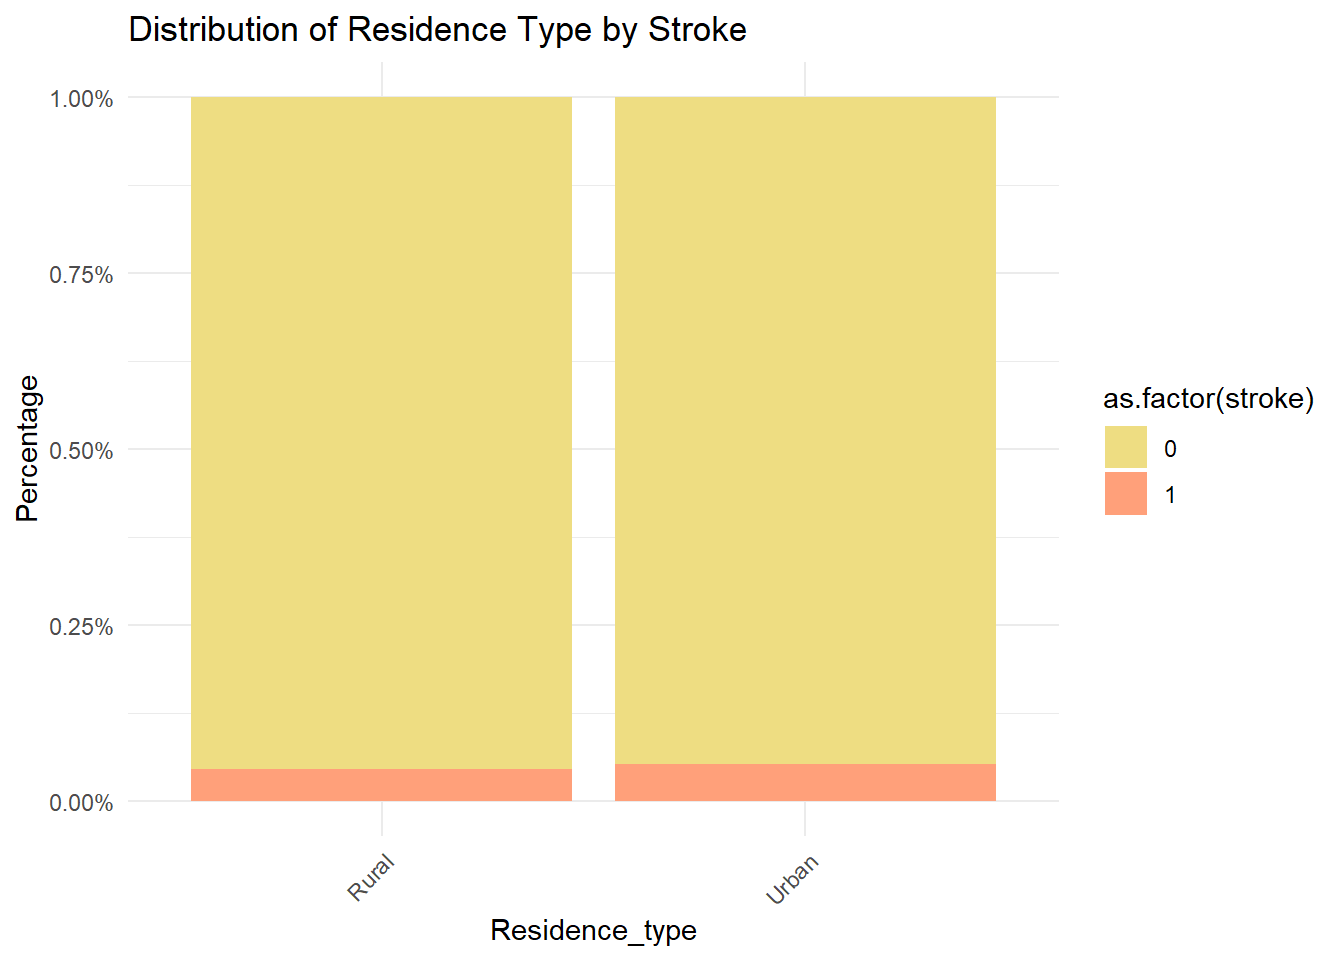
\includegraphics{Final_Project_files/figure-latex/unnamed-chunk-20-4.pdf}

\begin{Shaded}
\begin{Highlighting}[]
\CommentTok{\# Calculate the correlation matrix}
\NormalTok{cor\_matrix }\OtherTok{\textless{}{-}} \FunctionTok{cor}\NormalTok{(stroke[, }\FunctionTok{c}\NormalTok{(}\StringTok{"age"}\NormalTok{, }\StringTok{"avg\_glucose\_level"}\NormalTok{, }\StringTok{"bmi"}\NormalTok{)])}

\CommentTok{\# Plot the correlation matrix with an attractive color scale}
\FunctionTok{corrplot}\NormalTok{(cor\_matrix, }\AttributeTok{method =} \StringTok{"color"}\NormalTok{, }\AttributeTok{col =} \FunctionTok{colorRampPalette}\NormalTok{(}\FunctionTok{c}\NormalTok{(}\StringTok{"darkblue"}\NormalTok{, }\StringTok{"white"}\NormalTok{, }\StringTok{"darkred"}\NormalTok{))(}\DecValTok{100}\NormalTok{), }
         \AttributeTok{addCoef.col =} \StringTok{"black"}\NormalTok{, }\AttributeTok{tl.cex =} \FloatTok{0.8}\NormalTok{, }\AttributeTok{tl.srt =} \DecValTok{45}\NormalTok{)}
\end{Highlighting}
\end{Shaded}

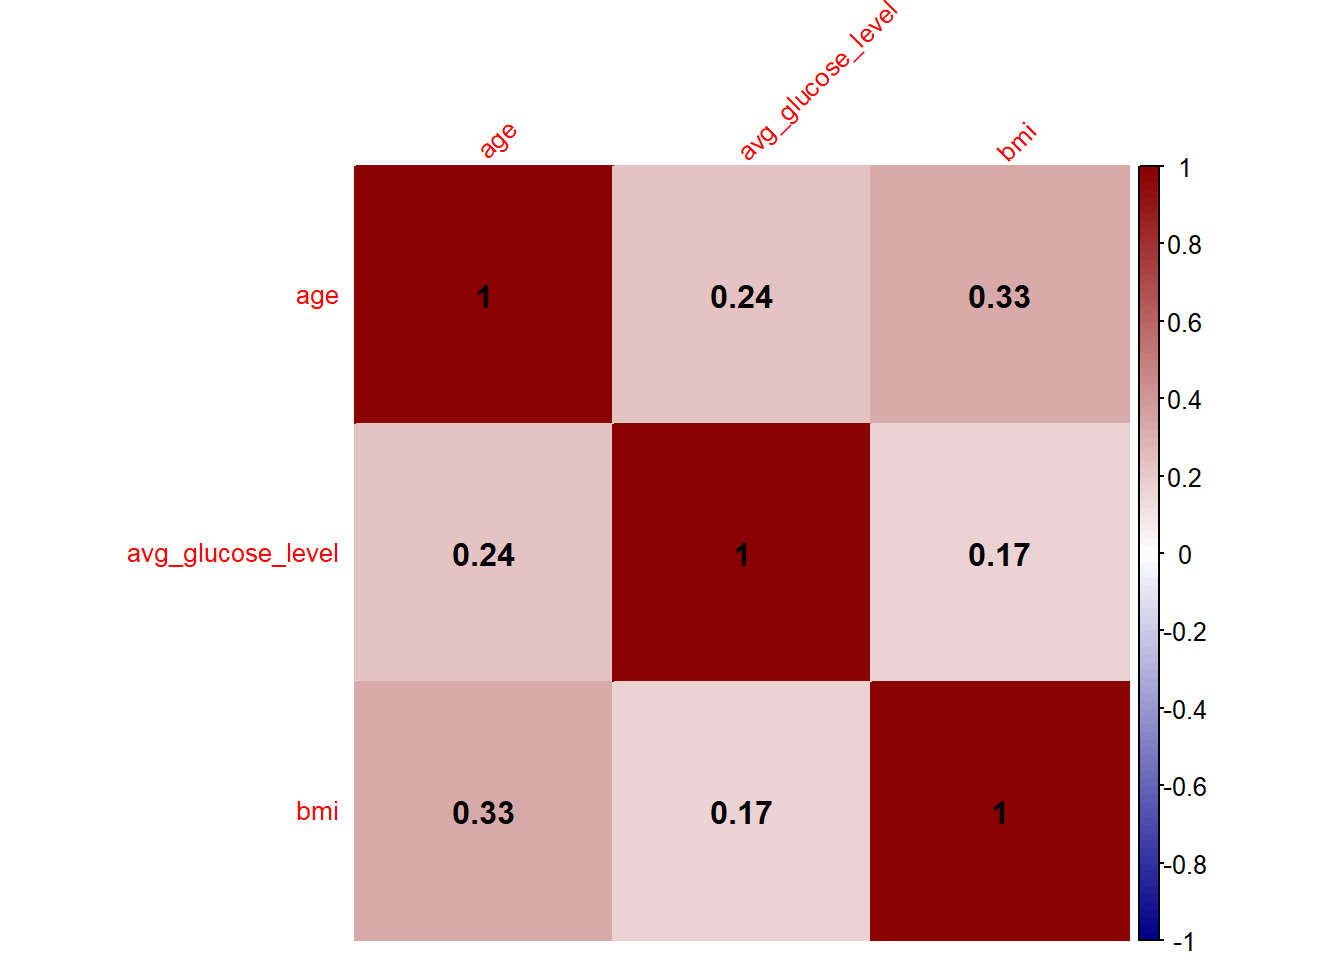
\includegraphics{Final_Project_files/figure-latex/unnamed-chunk-21-1.pdf}

\end{document}
